%%%%%%%%%%%%%%%%%%%% CHAPTER 3 %%%%%%%%%%%%%%%%%%%%%%%%%%
%%%%% Variables and Operators %%%%%%%%%%%%%%%%%%%%%%%%%%%%%%%%%%% 
\section{Simultaneous Linear Systems of Equations}
Many engineering simulations require the solution of simultaneous algebraic equations.
These algebraic equation systems are either linear or non-linear in the unknown variables.
Many computation schemes have been developed to solve the resulting systems, mostly depending on the structure of the systems (and the corresponding coefficient matrices).

The solution of linear (or non-linear for that matter) can be accomplished using either direct methods or iterative (successive approximation) methods. 
The method choice depends on:
\begin{enumerate}
\item The amount of computation required (size of the problem) and computer memory available.\footnote{In the past, the memory was indeed an issue -- its less so today; a really big problem of thousands of equations and thousands of variables might indeed be too big for any single computer array and would require out-of-core solver techniques, which I suspect are a slowly dying art.}
\item The accuracy of the solution required.
\item The ability to control accuracy (i.e. find accurate enough solutions) to improve overall computation speed and throughput.
\end{enumerate}
Direct solution methods lead to results by means of finite and predictable operations count, but at the expense of error amplification and  difficulty to deal with near-singular systems.  
Iterative methods can converge to exact solutions, are robust in near-singular cases, but at the expense of a non-predictable number of operations.   

In this chapter we will see how to solve systems using built-in method(s) in \textbf{R} and will also see the simplest of the iterative methods, Jacobi iteration.  
Jacobi iteration is presented for several reasons: it is simple to program, it shows the beauty of iteration when it works, and introduces a concept called pre-conditioning.
For problems in this workbook, the built in \texttt{solve(\dots)} is recomended; we will use Jacobi iteration later on the the aquifer flow models, because the model equation structure is quite amenable to this kind of solution method.  

For really large systems of equations iterative methods probably dominate because they are quite amenable to out-of-core solution --- Jacobi iteration is ideal for parallel processing in a GPU\footnote{Graphics Processing Unit --- Nearly all our laptops have GPU; either an Intel, NVIDIA, or AMD.  These are intended for rendering graphics, but can be directly accessed with the proper software tools and can perform floating point operations really quickly.   For example on my laptop I have an NVIDIA  GeForce GT750M which I can program using a CUDA toolkit.  If I had a really large system to solve, I would try Jacobi iteration, make each equation a thread, the solution guess a thread, and the update a thread.  Its relatively easy to multiply, add, and divide threads, so one could compute the update directly from parallel thread multiplication using the guess, then thread addition to update the guess, and repeat.  GPU programming is beyond this handbook, but remember that one can trade efficiency for speed if the operations are simple vector arithmetic.}


%%%%%%%%%%%%%%%%%%%%%%%%%% Matrix %%%%%%%%%%%%%%%%%%%%%%%%%%
%%%%%%%%%%%%%%%%%%%%%%%%%%%%%%%%%%%%%%%%%%%%%%%%%%%%%%%%%
\subsection{Numerical Linear Algebra -- Matrix Manipulation}
This section introduces use of matrices in \textbf{R} to learn how to address particular elements of a matrix -- once that is understood, the remaining arithmetic is reasonably straightforward.   
\subsection{The Matrix --- A data structure}
Listing \ref{lst:ReadMatrixNew} is script fragment that reads in two different matrices $\mathbf{A}$ and $\mathbf{B}$, and writes them back to the screen.   
While such an action alone is sort of meaningless, the code does illustrate how to read the two different files, and write back the result in a row wise fashion.

The two matrices are

\begin{gather}
\mathbf{A} =
\begin{pmatrix}
12 & 7 & 3 \\
~\\
4 & 5 &6 \\
~\\
7 & 8 & 9 \\
\end{pmatrix}
\end{gather}

and 

\begin{gather}
\mathbf{B} =
\begin{pmatrix}
5 & 8 & 1 & 2 \\
~\\
6 & 7 & 3 & 0 \\
~\\
4 & 5 & 9 & 1 \\
\end{pmatrix}
\end{gather}

Now that we have a way (albeit pretty arcane) for getting matrices into our program from a file\footnote{The read from a file is a huge necessity --- manually entering values will get old fast.   I have written matrix generators whose purpose in life is to construct matrices and put them into files for subsequent processing --- often these programs are pretty simple because of structure in a problem, at other times they rival the solution tool in complexity; once for a Linear Programming model (circa 1980's) I developed a code to write a 1200 X 1200 matrix to a file, which would be functionally impossible to enter by hand.} we can explore some elementary matrix arithmetic operations, and then will later move on to some more sophisticated operations, ultimately culminating in solutions to systems if linear equations (and non-linear systems in the next chapter).
\newpage
\begin{lstlisting}[caption=R code demonstrating reading in two matrices , label=lst:ReadMatrixNew]
# R script for some matrix operations
############## READ IN DATA FROM A FILE ####################
filepath <- "~/Dropbox/1-CE-TTU-Classes/CE4333-PCH-R/3-Readings/PCHinR-LectureNotes/5-LinearSystems/RScripts"
filename <- "MatrixA.txt"
fileToRead <- paste(filepath,filename,sep="/") # build the user absolute filename
# Read the first file
yy <- read.table(fileToRead,header=FALSE,sep=",") # comma seperated ASCII, No header
filename <- "MatrixB.txt"   # change the filename
fileToRead <- paste(filepath,filename,sep="/") # build the user absolute filename
# Read the second file
zz <- read.table(fileToRead,header=FALSE,sep=",") # comma seperated ASCII, No header
############## Get Row and Column Counts ###################
HowManyColumnsA <- length(yy)
HowManyRowsA    <- length(yy$V1)
HowManyColumnsB <- length(zz)
HowManyRowsB    <- length(zz$V1)
###############  Build A and B Matrices  ####################
Amat <- matrix(0,nrow = HowManyRowsA, ncol = HowManyColumnsA)
Bmat <- matrix(0,nrow = HowManyRowsB, ncol = HowManyColumnsB)
for (i in 1:HowManyRowsA){
  for(j in 1:(HowManyColumnsA)){
    Amat[i,j] <- yy[i,j]
  }
}
rm(yy) # deallocate zz and just work with matrix and vectors 
for (i in 1:HowManyRowsB){
  for(j in 1:(HowManyColumnsB)){
    Bmat[i,j] <- zz[i,j]
  }
}
rm(zz) # deallocate zz and just work with matrix and vectors 
############# Echo Input ###################################
print(Amat)
print(Bmat)
\end{lstlisting}

 
\subsection{Matrix Arithmetic}
Analysis of many problems in engineering result in systems of simultaneous equations.  
We typically represent systems of equations with a matrix.  
For example the two-equation system,

\begin{gather}
\begin{matrix}
2x_1 & ~+~~3x_2  \\
~\\
4x_1 & ~-~~3x_2 \\
\end{matrix}
\begin{matrix}
=~8\\
~\\
=~-2\\
\end{matrix}
\end{gather}

Could be represented by set of vectors and matrices\footnote{Usually called ``vector-matrix'' form.   Additionally, a vector is really just a matrix with column rank = 1 (a single column matrix).}

\begin{gather}
\mathbf{A} =
\begin{pmatrix}
2 & ~3 \\
~\\
4 & -3 \\
\end{pmatrix}
~
\mathbf{x} =
\begin{pmatrix}
x_1\\
~\\
x_2\\
\end{pmatrix}
~
\mathbf{b} =
\begin{pmatrix}
~8\\
~\\
-2\\
\end{pmatrix}
\end{gather}

and the linear system then written as

\begin{gather}
\mathbf{A} \cdot \mathbf{x} = \mathbf{b}
\end{gather}

So the ``algebra'' is considerably simplified, at least for writing things, 
however we now have to be able to do things like multiplication (indicated by $ ~\cdot $) as well as the concept of addition and subtraction, and division (multiplication by an inverse).  
There are also several kinds of matrix multiplication -- the inner product as required by the linear system, the vector (cross product), the exterior (wedge), and outer (tensor) product are a few of importance in both mathematics and engineering. 

The remainder of this section will examine the more common matrix operations.
\subsubsection{Matrix Definition}
A matrix is a rectangular array of numbers.
\begin{gather}
\begin{pmatrix}
1 & 5 & 7 & 2\\
2 & 9 & 17 & 5 \\
11 & 15 & 8 & 3 \\
\end{pmatrix}
\end{gather}

The size of a matrix is referred to in terms of the number of rows and the number of columns.  The enclosing parenthesis are optional above, but become meaningful when writing multiple matrices next to each other.
The above matrix is 3 by 4.  

When we are discussing matrices we will often refer to specific numbers in the matrix.  
To refer to a specific element of a matrix we refer to the row number (i) and the column number (j).  
We will often call a specific element of the matrix, the $a_{i,j}$ -th element of the matrix.  For example $a_{2,3}$ element in the above matrix is 17.  
In \textbf{R} we would refer to the element as \texttt{a\_matrix[i][j]} or whatever the name of the matrix is in the program.

\subsubsection{Multiply a matrix by a scalar}
A scalar multiple of a matrix is simply each element of the matrix multiplied by the scalar value.
 Consider the matrix $\mathbf{A}$ below.
\begin{gather}
\mathbf{A}=
\begin{pmatrix}
12 & 7 & 3 \\
4 & 5 &6 \\
7 & 8 & 9 \\
\end{pmatrix}
\end{gather}

If the scalar is say 2, then $2 \times \mathbf{A}$ is computed by doubling each element of $\mathbf{A}$, as

\begin{gather}
2\mathbf{A}=
\begin{pmatrix}
24 & 14 & 6\\
8 & 10 & 12 \\
17 & 16 & 18 \\
\end{pmatrix}
\end{gather}

In \textbf{R} we can simply perform the arithmetic as

\begin{lstlisting}[caption=R code demonstrating scalar multiplication , label=lst:ScalarMultiply]
#######################
twoA <- 2 * Amat
print(twoA)
\end{lstlisting}


Figure \ref{fig:ScalarMultiply} is an example using the earlier $\mathbf{A}$ matrix and multiplying it by the scalar value of 2.0.   

\begin{figure}[h!] %  figure placement: here, top, bottom, or page
   \centering
   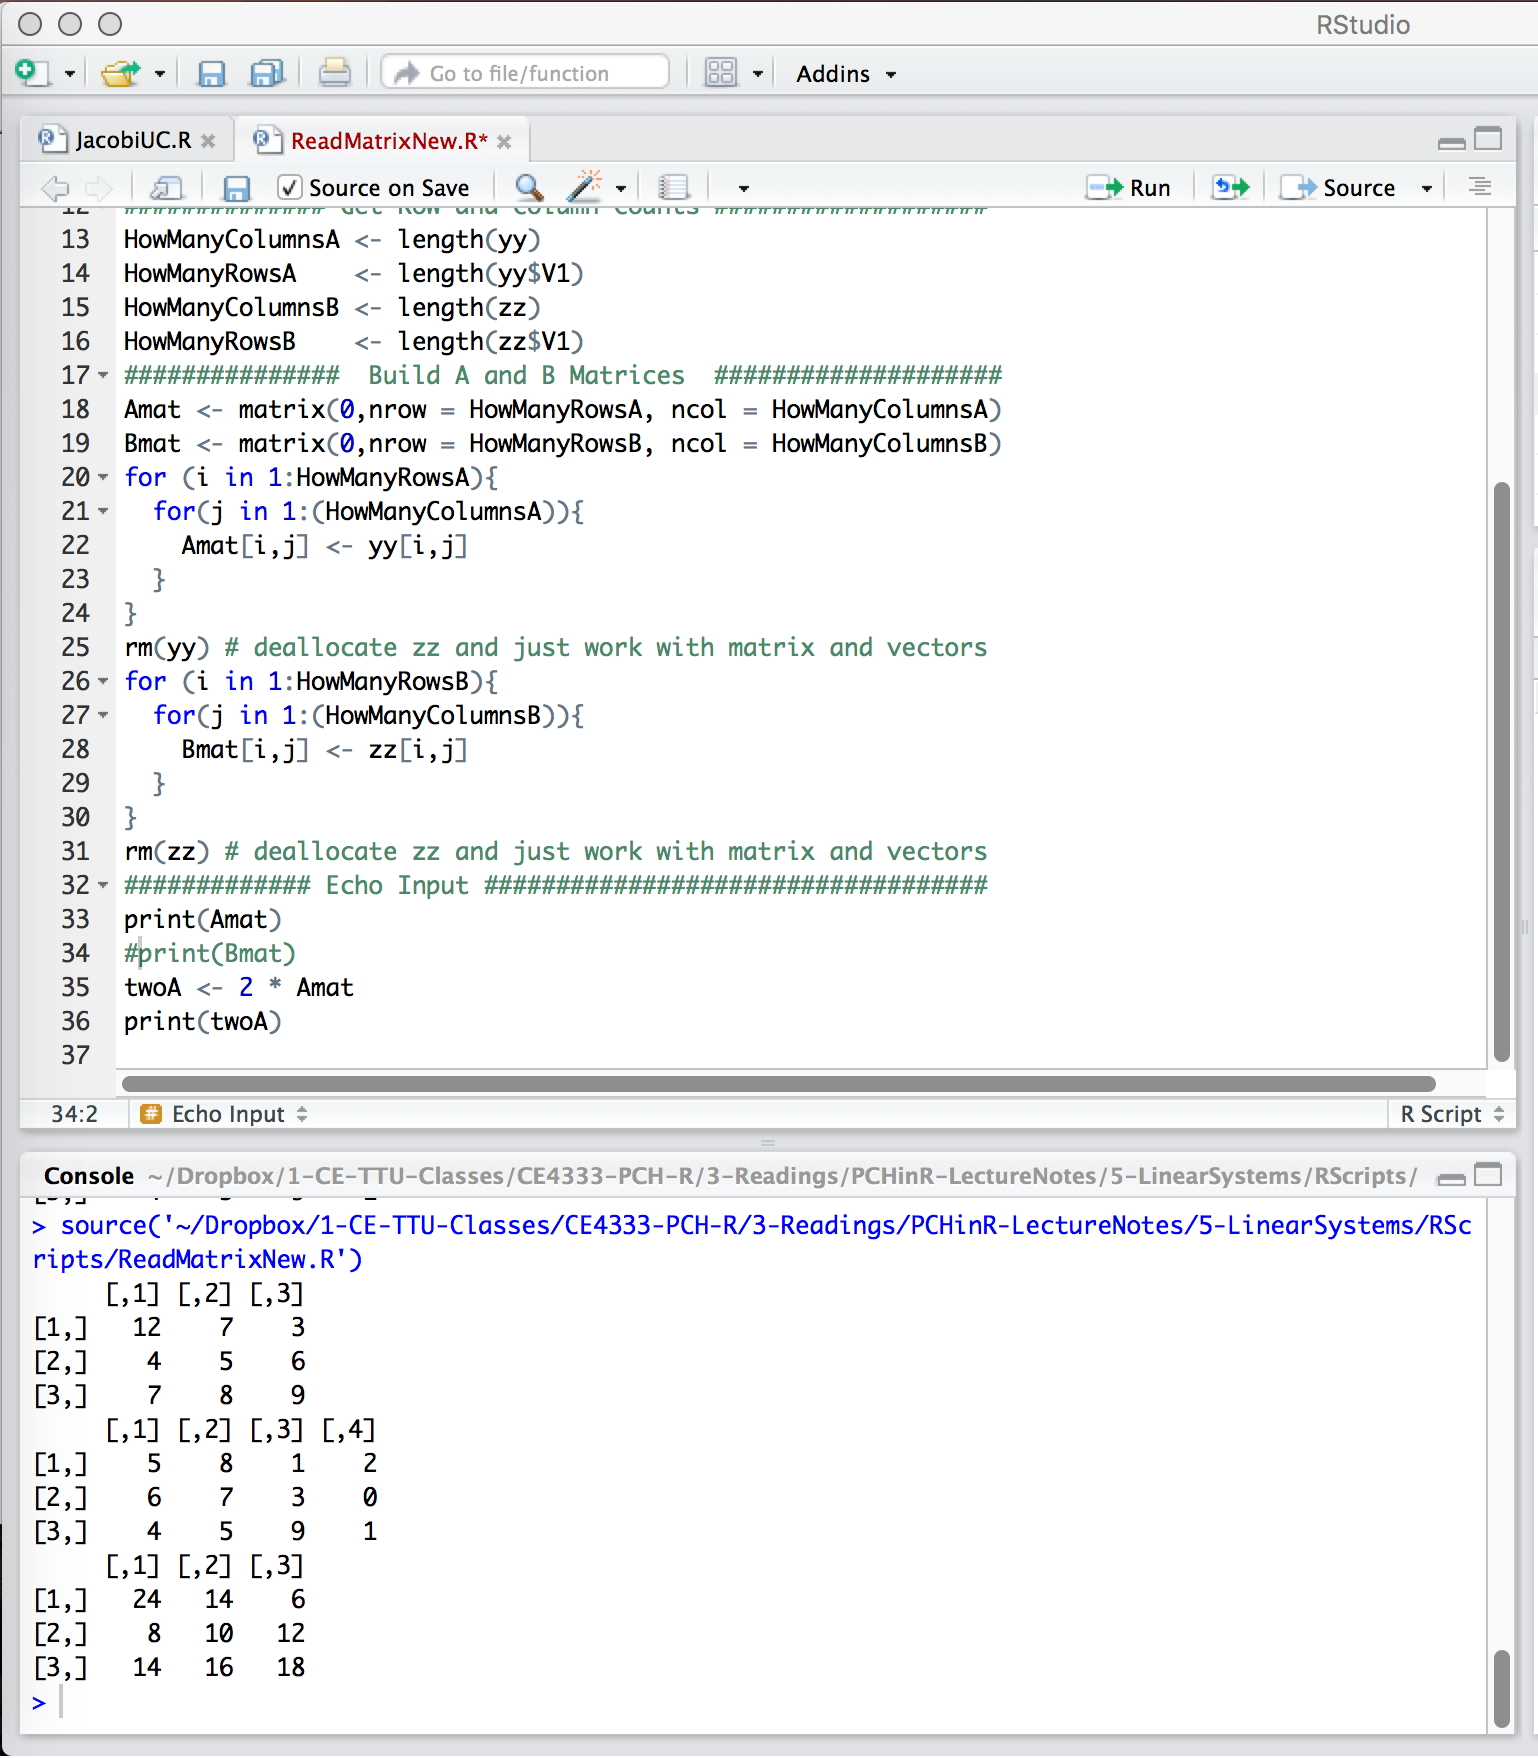
\includegraphics[width=6in]{./5-LinearSystems/ScalarMultiply.jpg} 
   \caption{Multiply each element in \texttt{amatrix} by a scalar }
   \label{fig:ScalarMultiply}
\end{figure}

\clearpage
 \subsubsection{Matrix addition (and subtraction)}
Matrix addition and subtraction are also element-by-element operations.
In order to add or subtract two matrices they must be the same size and shape.  
This requirement means that they must have the same number of rows and columns.  
To add or subtract a matrix we simply add or subtract the corresponding elements from each matrix.

For example consider the two matrices $\mathbf{A}$ and $\mathbf{2A}$ below


\begin{gather}
\mathbf{A}=
\begin{pmatrix}
12 & 7 & 3 \\
4 & 5 &6 \\
7 & 8 & 9 \\
\end{pmatrix}
~ 
2\mathbf{A}=
\begin{pmatrix}
24 & 14 & 6\\
8 & 10 & 12 \\
17 & 16 & 18 \\
\end{pmatrix}
\end{gather}

For example the sum of these two matrices is the matrix named $\mathbf{3A}$,  shown below:

\begin{gather}
\mathbf{A+2A}=
\begin{pmatrix}
12+24 & 7+14 & 3+6 \\
4+8 & 5+10 & 6+12 \\
7+14 & 8+16 & 9+18 \\
\end{pmatrix}
=
\begin{pmatrix}
36 &  21 &   9 \\
12  & 15 &  18 \\
21  & 24 &  27 \\
\end{pmatrix}
\end{gather}

Now to do the operation in \textbf{R}, we need to read in the matrices, perform the addition, and write the result.  
In the code example in \ref{fig:AddMatrix} I added a third matrix to store the result -- generally we don't want to clobber existing matrices, so we will use the result instead.   

\begin{figure}[h!] %  figure placement: here, top, bottom, or page
   \centering
   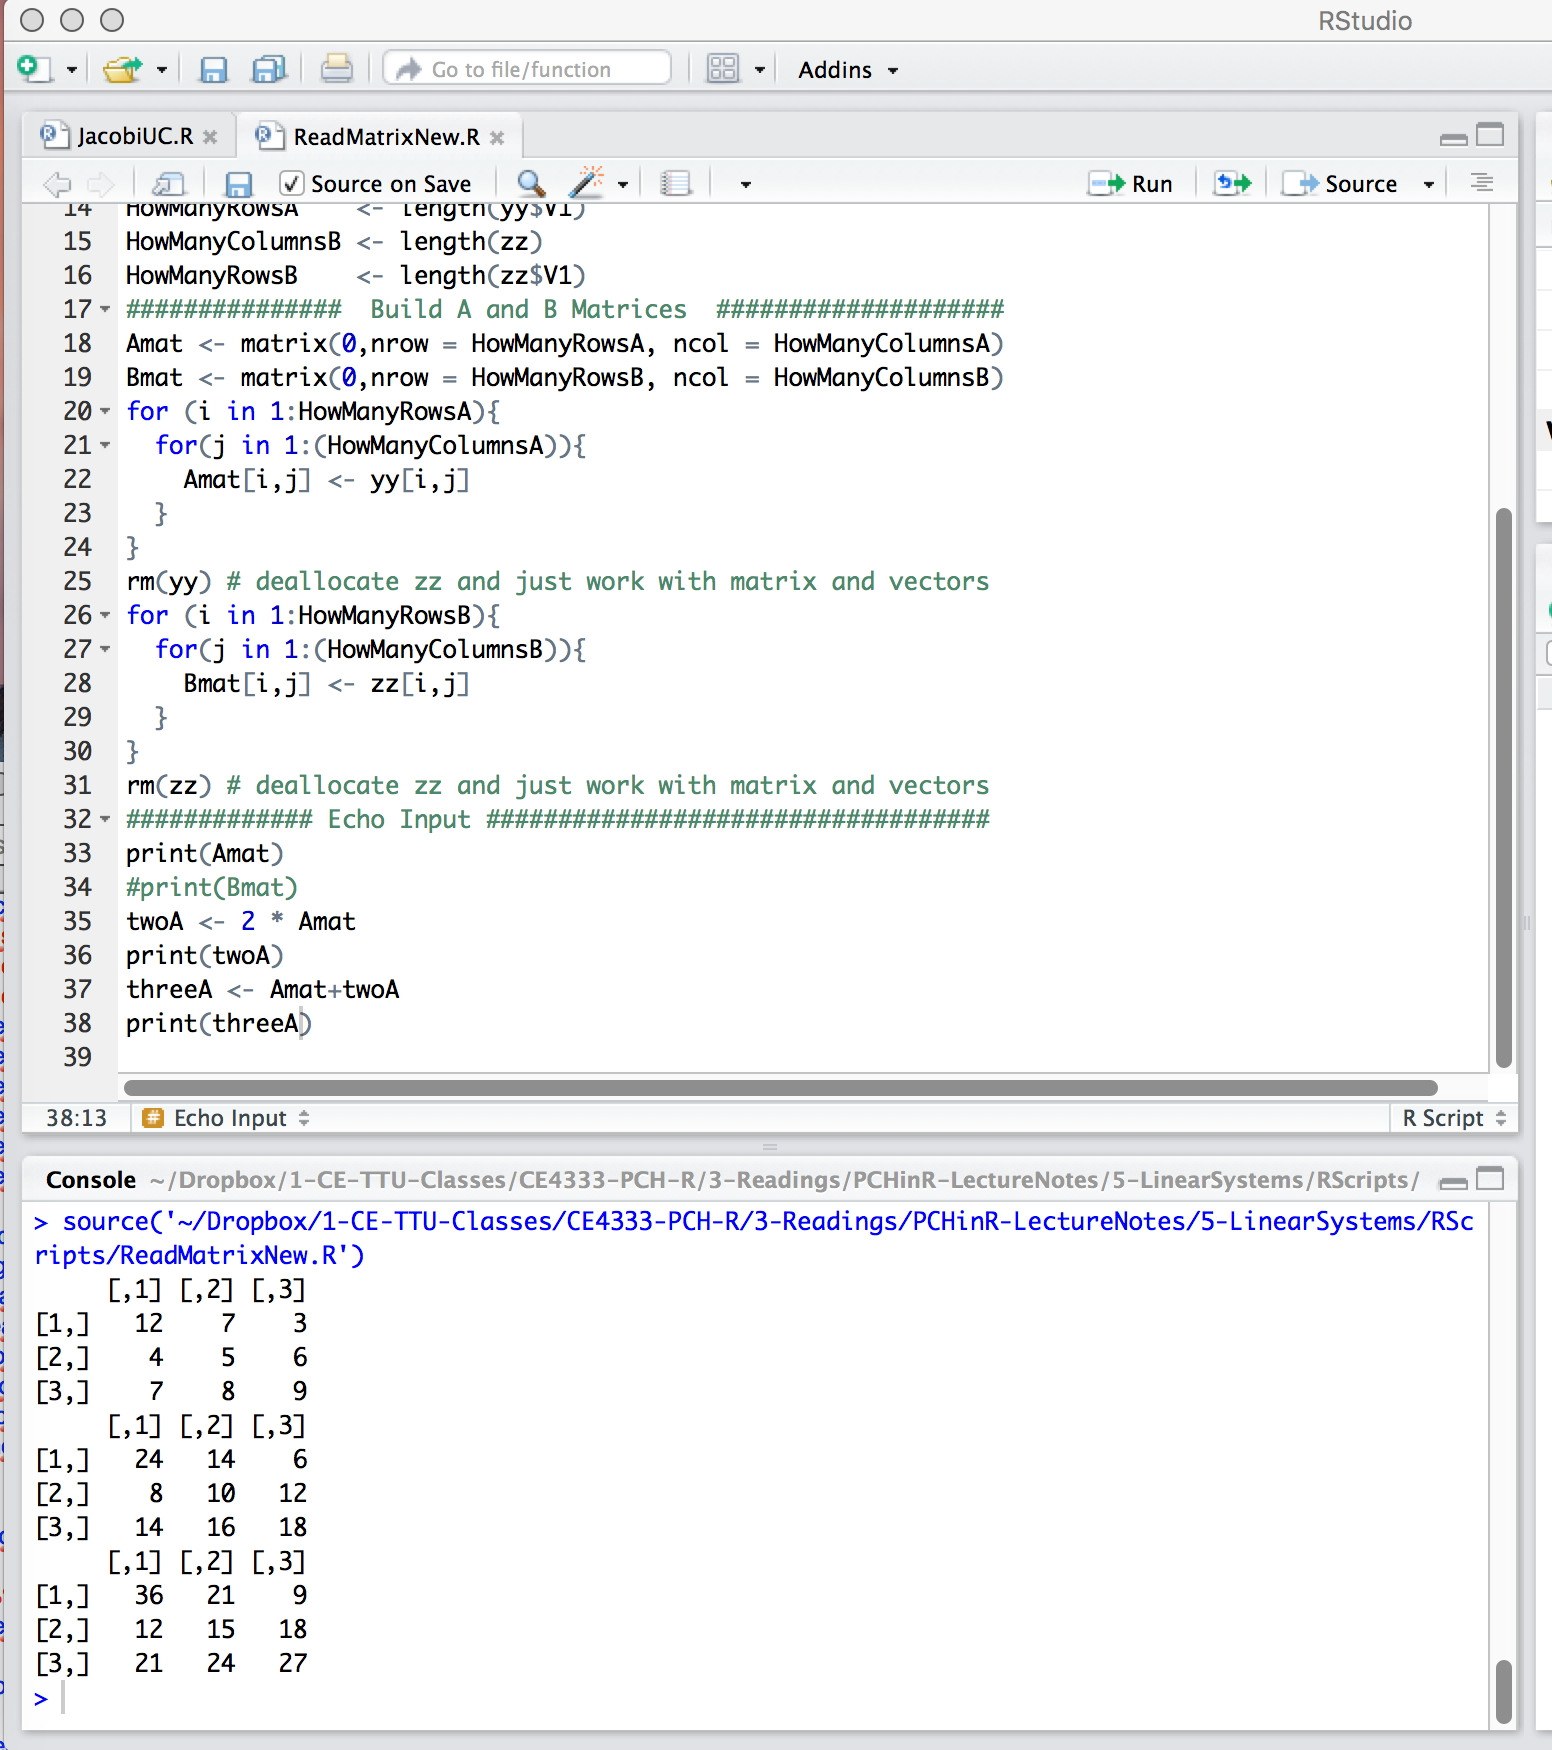
\includegraphics[width=6in]{./5-LinearSystems/AddMatrix.jpg} 
   \caption{Add each element in \texttt{A} to each element in \texttt{twoA}, store the result in \texttt{threeA}.}
   \label{fig:AddMatrix}
\end{figure}

Subtraction is performed in a similar fashion, except the subtraction operator is used.  
\clearpage
\subsubsection{Multiply a matrix}
One kind of matrix multiplication is an inner product.  
Usually when matrix multiplication is mentioned without further qualification ,the implied meaning is an inner product of the matrix and a vector (or another matrix).

Matrix multiplication is  more complex than addition and subtraction.  
If two matrices such as a matrix $\mathbf{A}$ (size l x m) and a matrix $\mathbf{B}$ ( size m x n) are multiplied together, the resulting matrix $\mathbf{C}$ has a size of l x n.  
The order of multiplication of matrices is extremely important\footnote{Matrix multiplication is not  transitive;  $\mathbf{A}~\mathbf{B} ~\ne~  \mathbf{B}~\mathbf{A}$.}.  

To obtain $\mathbf{C}$ = $\mathbf{A}$ $\mathbf{B}$, the number of columns in $\mathbf{A}$ must be the same as the number of rows in $\mathbf{B}$.  In order to carry out the matrix operations for multiplication of matrices, the $i,j$-th element of  $\mathbf{C}$ is simply equal to the scalar (dot or inner) product of row $i$ of $\mathbf{A}$ and column $j$ of $\mathbf{B}$.

Consider the example below
\begin{gather}
\mathbf{A}=
\begin{pmatrix}
1 & 5 & 7 \\
2 & 9 & 3 \\
\end{pmatrix}
~ 
\mathbf{B}=
\begin{pmatrix}
3 & -2  \\
-2 & 1 \\
1 & 1 \\
\end{pmatrix}
\end{gather}

First, we would evaluate if the operation is even possible, $\mathbf{A}$ has two rows and three columns.  
$\mathbf{B}$ has three rows and two columns.  
By our implied multiplication ``rules'' for the multiplication to be defined the first matrix must have the same number of rows as the second matrix has columns (in this case it does), and the result matrix will have the same number of rows as the first matrix, and the same number of columns as the second matrix (in this case the result will be a 2X2 matrix).

\begin{gather}
\mathbf{C}=\mathbf{A}\mathbf{B}=
\begin{pmatrix}
c_{1,1} & c_{1,2} \\
c_{2,1} & c_{2,2} \\
\end{pmatrix}
\end{gather}

And each element of $\mathbf{C}$ is the dot product of the row vector of $\mathbf{A}$ and the column vector of $\mathbf{B}$.
\newpage

\begin{gather}
c_{1,1} =
\begin{pmatrix}
1 & 5 & 7 \\
\end{pmatrix}
\cdot
\begin{pmatrix}
3 \\
-2 \\
1 \\
\end{pmatrix}
=
\begin{pmatrix}
(1)(3) +(5)(-2) + (7)(1)\\
\end{pmatrix}
= 0
\end{gather}

\begin{gather}
c_{1,2} =
\begin{pmatrix}
1 & 5 & 7 \\
\end{pmatrix}
\cdot
\begin{pmatrix}
-2 \\
1 \\
1 \\
\end{pmatrix}
=
\begin{pmatrix}
(1)(-2) +(5)(1) + (7)(1)\\
\end{pmatrix}
= 10
\end{gather}


\begin{gather}
c_{2,1} =
\begin{pmatrix}
2 & 9 & 3 \\
\end{pmatrix}
\cdot
\begin{pmatrix}
3 \\
-2 \\
1 \\
\end{pmatrix}
=
\begin{pmatrix}
(2)(3) +(9)(-2) + (3)(1)\\
\end{pmatrix}
= -9
\end{gather}


\begin{gather}
c_{2,2} =
\begin{pmatrix}
2 & 9 & 3 \\
\end{pmatrix}
\cdot
\begin{pmatrix}
-2 \\
1 \\
1 \\
\end{pmatrix}
=
\begin{pmatrix}
(2)(-2) +(9)(1) + (3)(1)\\
\end{pmatrix}
= 8
\end{gather}

Making the substitutions results in :

\begin{gather}
\mathbf{C}=\mathbf{A}\mathbf{B}=
\begin{pmatrix}
0 & 10 \\
-9 & 8 \\
\end{pmatrix}
\end{gather}

So in an algorithmic sense we will have to deal with three matrices, the two source matrices and the destination matrix.  
We will also have to manage element-by-element multiplication and be able to correctly store through rows and columns.
In \textbf{R} this manipulation is handled for us by the matrix multiply operator \texttt{\% * \%}. 

Figure \ref{fig:MultiplyMatrix} is a script that multiplies the two matrices above and prints the result.\footnote{Internal to \textbf{R} the actual code for the multiplication is three nested for-loops.  The outer loop counts based rows of the first matrix, the middle loop counts based on columns of the second matrix, and the inner most loop counts based on columns of the first matrix ( or rows of the second matrix).   In many practical cases we may actually have to manipulate at the element level --- similar to how the \texttt{zz} object was put into a matrix explicitly above.}   

\begin{figure}[h!] %  figure placement: here, top, bottom, or page
   \centering
   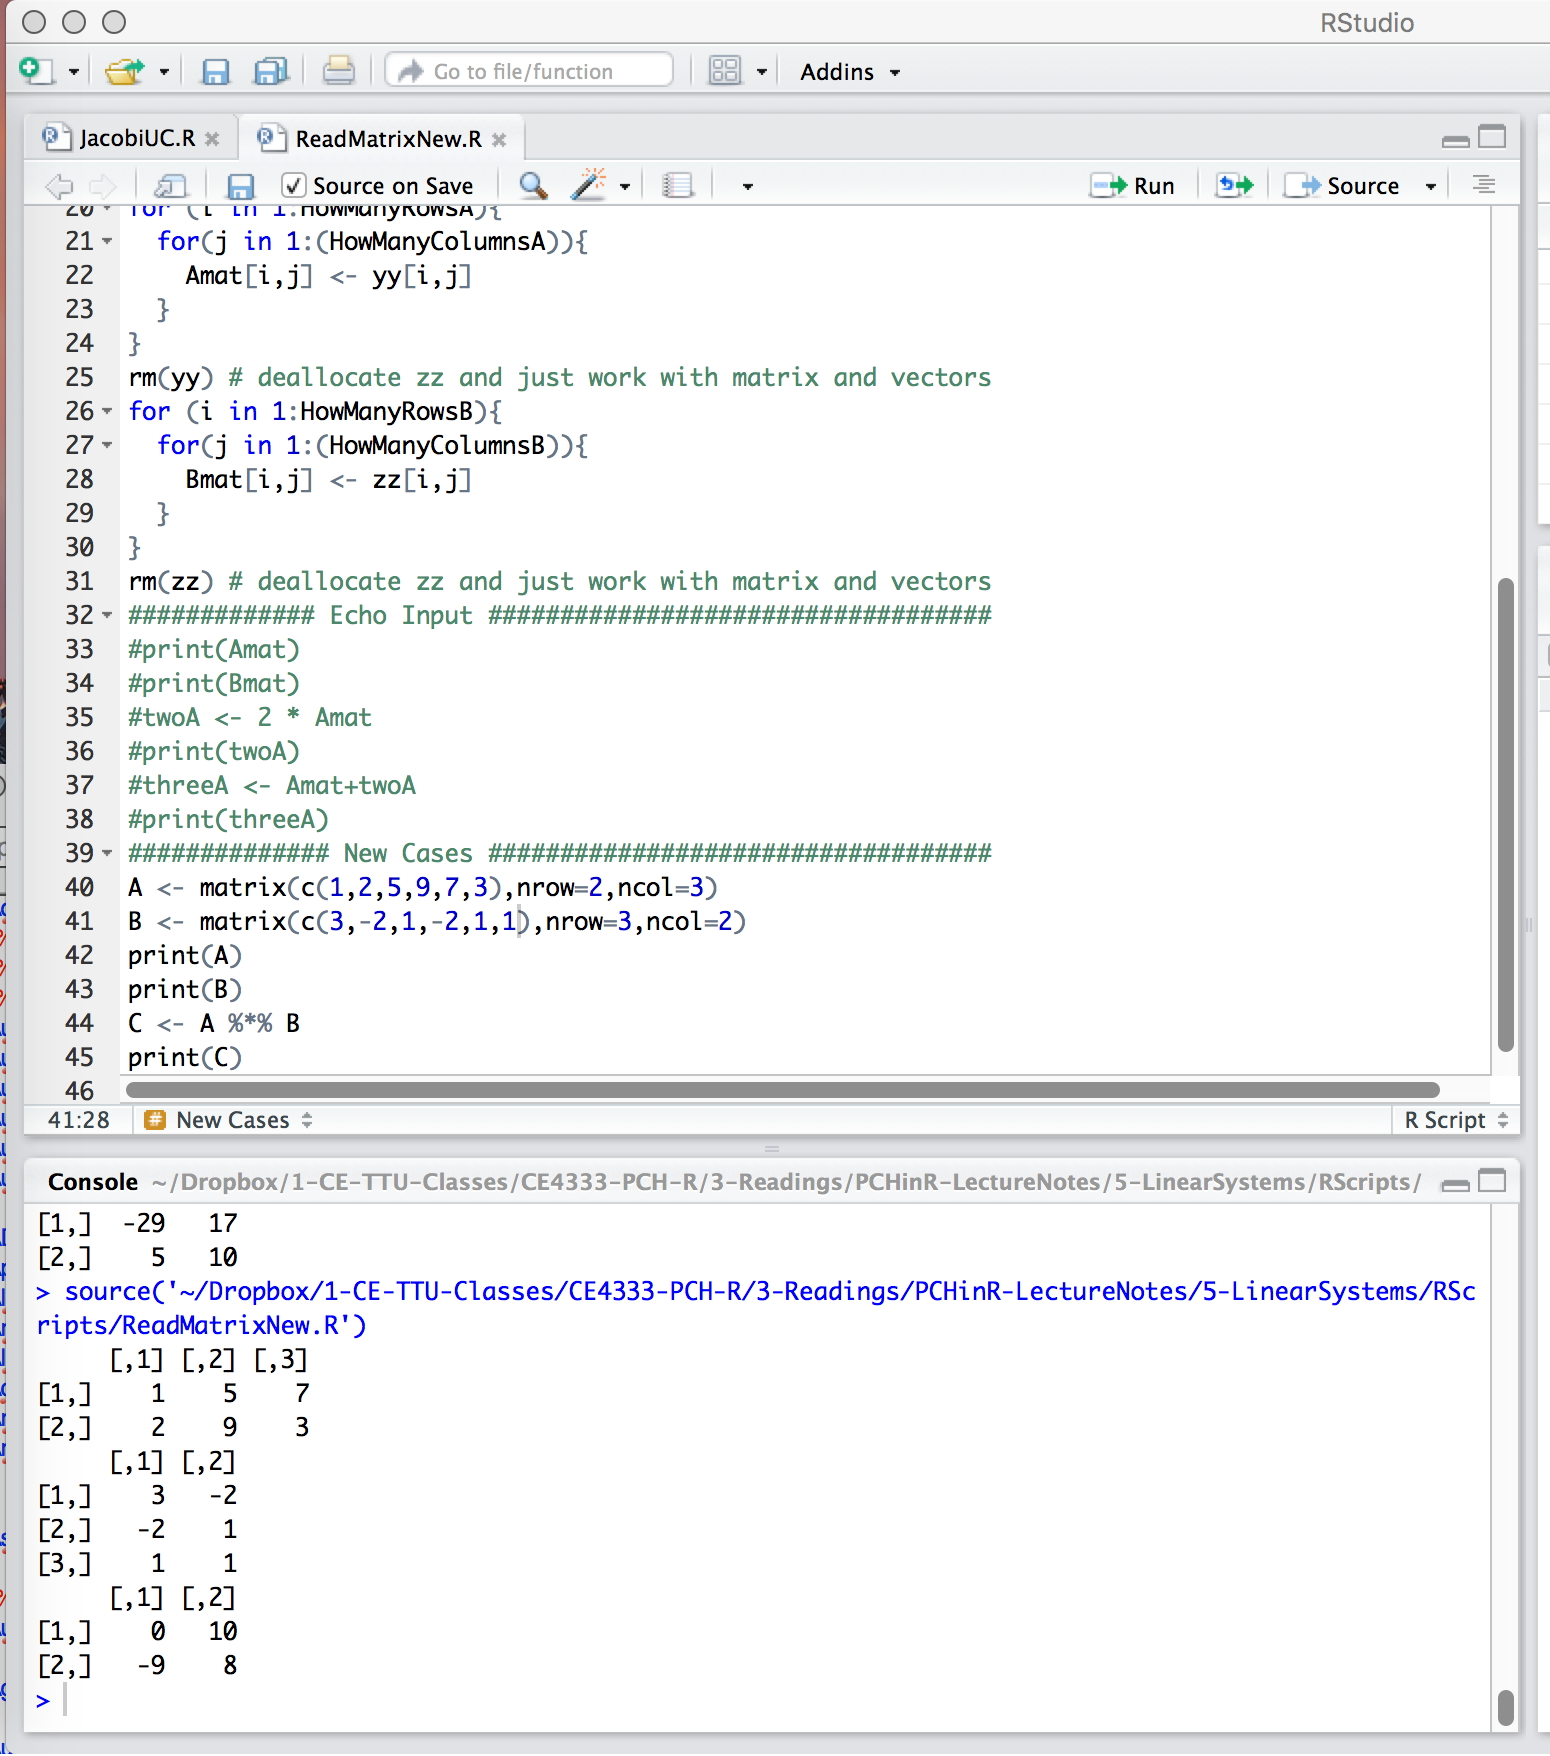
\includegraphics[width=6in]{./5-LinearSystems/MultiplyMatrix.jpg} 
   \caption{Matrix multiplication example}
   \label{fig:MultiplyMatrix}
\end{figure}

\subsubsection{Identity matrix}
In computational linear algebra we often need to make use of a special matrix called the ``Identity Matrix''.  
The Identity Matrix is a square matrix with all zeros except the $i,i$0-th element (diagonal) which is equal to 1:

\begin{gather}
\mathbf{I}_{3\times3}=
\begin{pmatrix}
1 & 0 & 0\\
0 & 1 & 0\\
0 & 0 & 1\\
\end{pmatrix}
\end{gather}
Usually we don't bother with the size subscript i used above and just stipulate that the matrix is sized as appropriate.
Multiplying any matrix by (a correctly sized) identity matrix results in no change in the matrix.  $\mathbf{I}\mathbf{A} = \mathbf{A}$  

In \textbf{R} the identity matrix is easily created using \texttt{$<$matrix\_name$>$~$<$- diag(dimension)}.

\subsubsection{Matrix Inverse}
In many practical computational and theoretical operations we employ the concept of the inverse of a matrix.
The inverse is somewhat analogous to``dividing'' by the matrix.  
Consider our linear system 
\begin{gather}
\mathbf{A} \cdot \mathbf{x} = \mathbf{b}
\end{gather}
If we wished to solve for $\mathbf{x}$ we would ``divide'' both sides of the equation by $\mathbf{A}$.   
Instead of division (which is essentially left undefined for matrices) we instead multiply by the inverse of the matrix\footnote{The matrix inverse is the multiplicative inverse of the matrix -- we are defining the equivalent of a division operation, just calling it something else.  This issue will be huge later on in our workbook, especially when we are dealing with non-linear systems}.
The inverse of a matrix $\mathbf{A}$ is denoted by $\mathbf{A}^{-1}$ and by definition is a matrix such that when $\mathbf{A}^{-1}$ and $\mathbf{A}$ are multiplied together, the identity matrix $\mathbf{I}$ results.  e.g. $\mathbf{A}^{-1} \mathbf{A} = \mathbf{I}$

Lets consider the matrixes below
\begin{gather}
\mathbf{A}=
\begin{pmatrix}
2 & 3 \\
4 & -3 \\
\end{pmatrix}
\end{gather}

\begin{gather}
\mathbf{A}^{-1}=
\begin{pmatrix}
\frac{1}{6} & \frac{1}{6} \\
~\\
\frac{2}{9} & -\frac{1}{9} \\
\end{pmatrix}
\end{gather}

We can check that the matrices are indeed inverses of each other using \textbf{R} and matrix multiplication --- it should return an identity matrix.
  
Figure \ref{fig:InverseMatrixCheck} is our multiplication script modified where $\mathbf{A} = \mathbf{A} $ and $\mathbf{B} = \mathbf{A}^{-1}$
perform the multiplication and then report the result.   
The result is the identity matrix regardless of the order of operation.\footnote{Why do you think this is so, when above we stated that multiplication is intransitive?}

\begin{figure}[h!] %  figure placement: here, top, bottom, or page
   \centering
   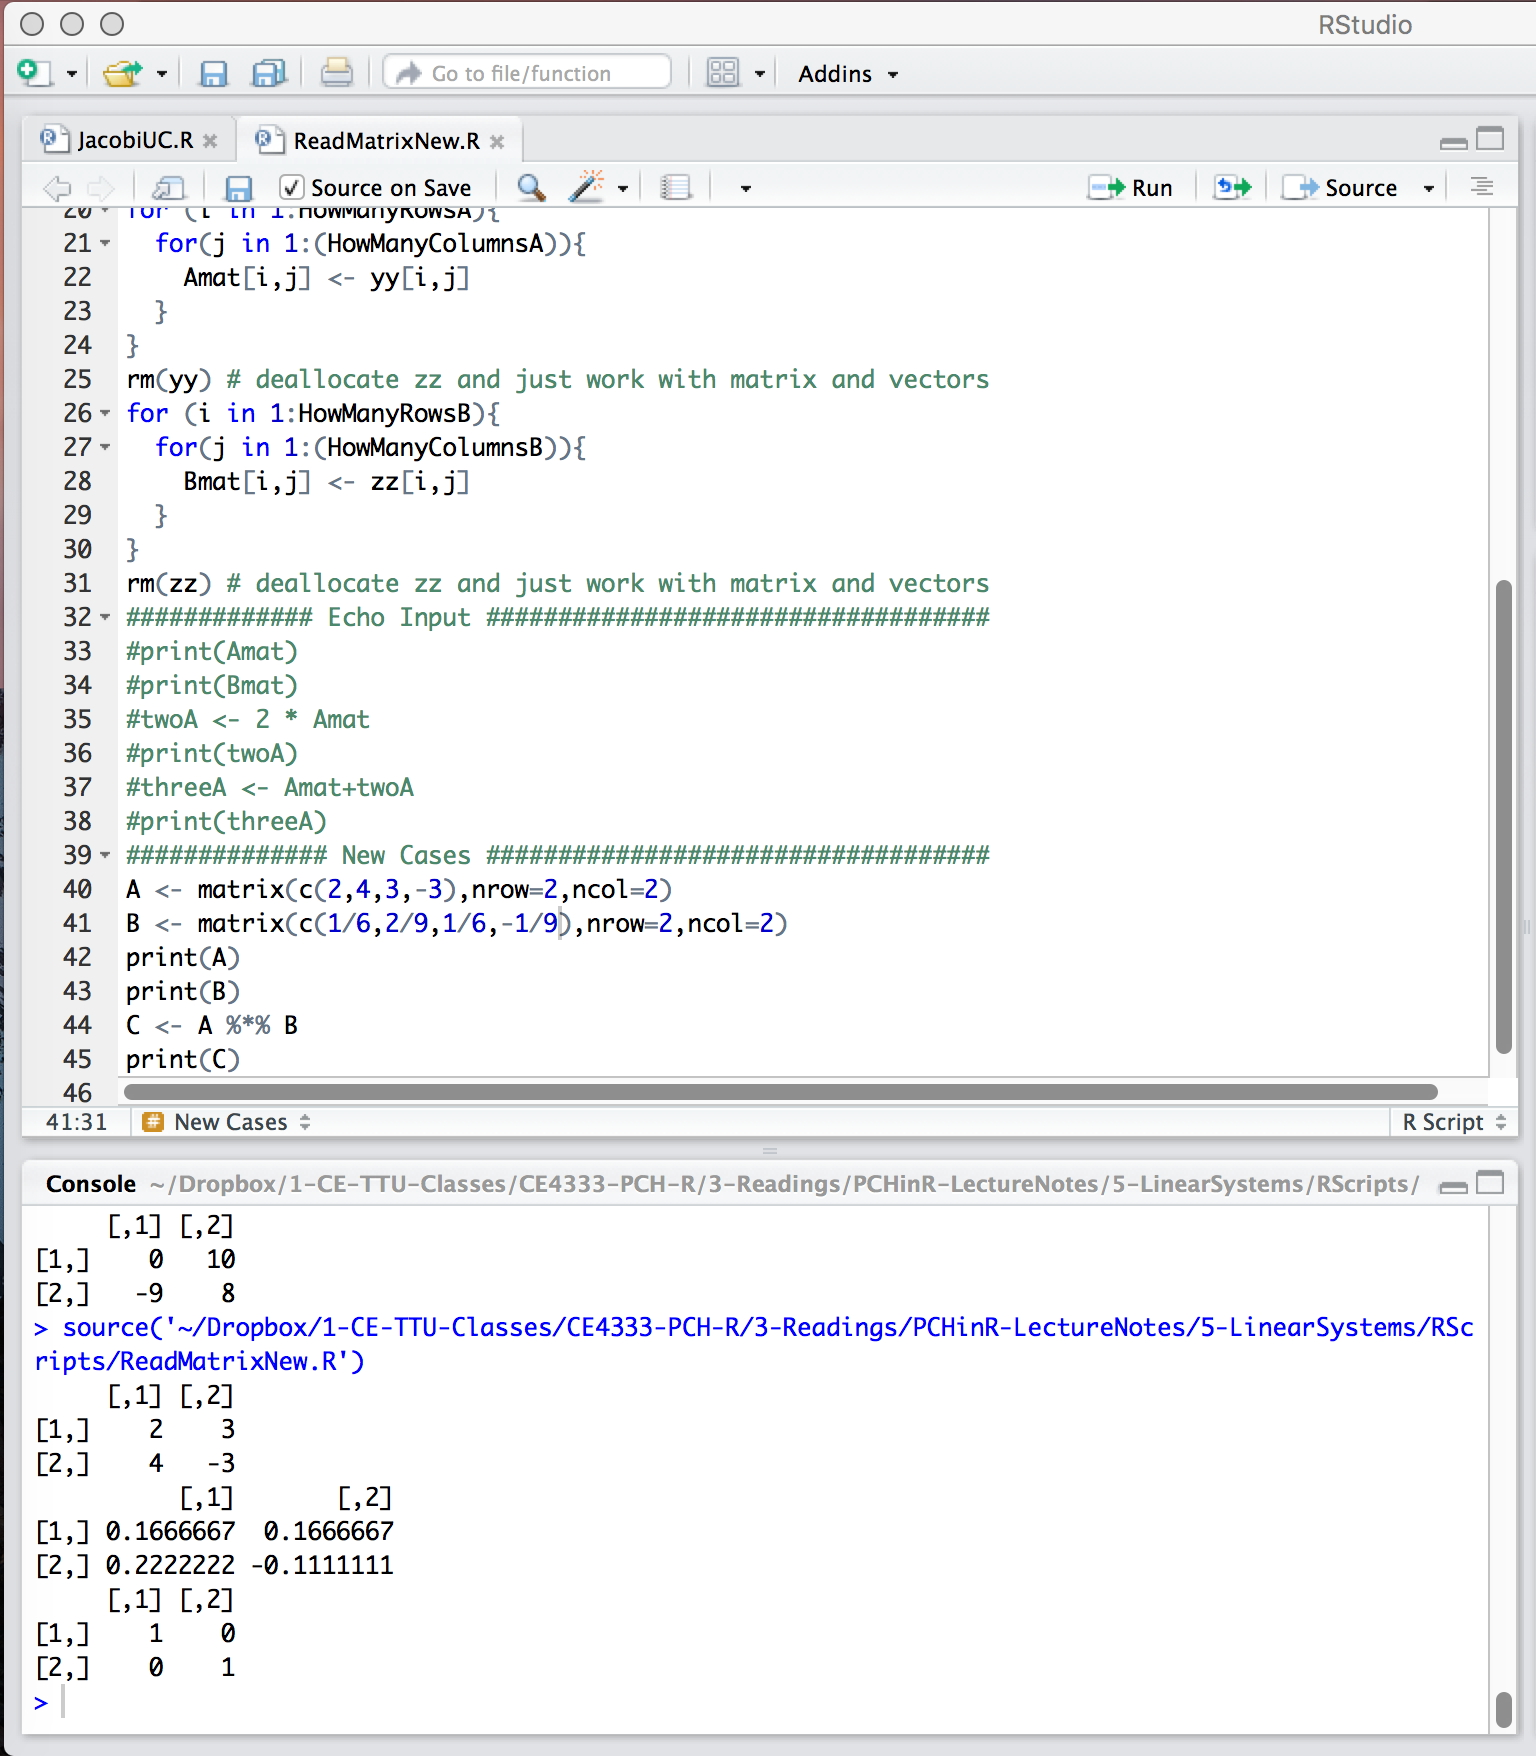
\includegraphics[width=6in]{./5-LinearSystems/InverseMatrixCheck.jpg} 
   \caption{Matrix multiplication used to check an inverse.}
   \label{fig:InverseMatrixCheck}
\end{figure}

Now that we have some background on what an inverse is, it would be nice to know how to find them --- that is a remarkably challenging problem.   Here we examine a classical algorithm for finding an inverse if we really need to --- computationally we only invert if necessary, there are other ways to ``divide'' that are faster.

\subsubsection{Gauss-Jordan method of finding $\mathbf{A}^{-1}$}
There are a number of methods that can be used to find the inverse of a matrix using elementary row operations.  
An elementary row operation is any one of the three operations listed below:
\begin{enumerate}
\item Multiply or divide an entire row by a constant.
\item Add or subtract a multiple of one row to/from another.
\item Exchange the position of any 2 rows.
\end{enumerate}

The Gauss-Jordan method of inverting a matrix can be divided into 4 main steps.  
In order to find the inverse we will be working with the original matrix, augmented with the identity matrix -- this new matrix is called the augmented matrix (because no-one has tried to think of a cooler name yet).  

\begin{gather}
\mathbf{A} | \mathbf{I} =
\begin{pmatrix}
2 & 3 & | & 1 & 0 \\
4 & -3 & | & 0 & 1 \\
\end{pmatrix}
\end{gather}

We will perform elementary row operations based on the left matrix to convert it to an identity matrix -- we perform the same operations on the right matrix and the result when we are done is the inverse of the original matrix.

So here goes -- in the theory here, we also get to do infinite-precision arithmetic, no rounding/truncation errors.  

\begin{enumerate}
\item Divide row one by the $a_{1,1}$ value to force a $1$ in the $a_{1,1}$ position.   This is elementary row operation 1 in our list above.
\begin{gather}
\mathbf{A} | \mathbf{I} =
\begin{pmatrix}
2/2 & 3/2 & | & 1/2 & 0 \\
4 & -3 & | & 0 & 1 \\
\end{pmatrix}
=
\begin{pmatrix}
1 & 3/2 & | & 1/2 & 0 \\
4 & -3 & | & 0 & 1 \\
\end{pmatrix}
\end{gather}

\item For all rows below the first row, replace $row_j$ with $row_j - a_{j,1}*row_1$.  
This happens to be elementary row operation 2 in our list above.
\begin{gather}
\mathbf{A} | \mathbf{I} =
\begin{pmatrix}
1 & 3/2 & | & 1/2 & 0 \\
4 - 4(1) & -3 - 4(3/2) & | & 0-4(1/2) & 1-4(0) \\
\end{pmatrix}
=
\begin{pmatrix}
1 & 3/2 & | & 1/2 & 0 \\
0 & -9 & | & -2 & 1 \\
\end{pmatrix}
\end{gather}


\item Now multiply $row_2$ by $ \frac{1}{ a_{2,2}} $.  This is again elementary row operation 1 in our list above.

\begin{gather}
\mathbf{A} | \mathbf{I} =
\begin{pmatrix}
1 & 3/2 & | & 1/2 & 0 \\
0 & -9/-9 & | & -2/-9 & 1/-9 \\
\end{pmatrix}
=
\begin{pmatrix}
1 & 3/2 & | & 1/2 & 0 \\
0 & 1 & | & 2/9 & -1/9 \\
\end{pmatrix}
\end{gather}

\item For all rows above and below this current row, replace $row_j$ with $row_j - a_{2,2}*row_2$.  
This happens to again be elementary row operation 2 in our list above.  
What we are doing is systematically converting the left matrix into an identity matrix by multiplication of constants and addition to eliminate off-diagonal values and force 1 on the diagonal.

\begin{gather}
\mathbf{A} | \mathbf{I} = \\
\begin{pmatrix}
1 & 3/2 - (3/2)(1) & | & 1/2 - (3/2)(2/9) & 0-(3/2)(-1/9) \\
0 & 1 & | & 2/9 & -1/9 \\
\end{pmatrix}
= \\
\begin{pmatrix}
1 & 0 & | & 1/6 & 1/6 \\
0 & 1 & | & 2/9 & -1/9 \\
\end{pmatrix}
\end{gather}

\item As far as this example is concerned we are done and have found the inverse.  
With more than a 2X2 system there will be many operations moving up and down the matrix to eliminate the off-diagonal terms.
\end{enumerate}
So the next logical step is to build an algorithm to perform these operations for us.  

In \textbf{R} inversion is simply performed using the \texttt{solve(\dots)} function where the only argument passed to the function is the matrix.\footnote{If we have to write code ourselves, its not terribly hard, but is lengthy and consequently error-prone. Sometimes we have no choice, but in this workbook, we will use the built-in tool as much as possible.  \textbf{R} does not use Gaussian reduction unless we tell it to do so, it implements a factorization called LU (or Cholesky) decomposition, then computes the inverse by repeated solution of a linear system with the right hand side being selected from one of the identify matrix columns (as was done above).}

Figure \ref{fig:InvertedMatrix} is a screen capture of using \texttt{solve(\dots)} to find the inverse of \textbf{A}.  The result is identical to the input matrix \textbf{A$^{-1}$} above.   
While we now have the ability to solve linear systems by rearrangement into 
\begin{gather}
\mathbf{x} = \mathbf{A^{-1}} \cdot \mathbf{b}
\end{gather}
this is generally not a good approach (we are solving $n$ linear systems to obtain the inverse, instead of only the one we seek!).

Instead to solve a linear system, we would supply the coefficient matrix $\mathbf{A}$ and the right hand side $\mathbf{b}$, and then supply these two matrices to the solve routine \\ (e.g.~ \texttt{x <- solve(A,b)}).

\begin{figure}[h!] %  figure placement: here, top, bottom, or page
   \centering
   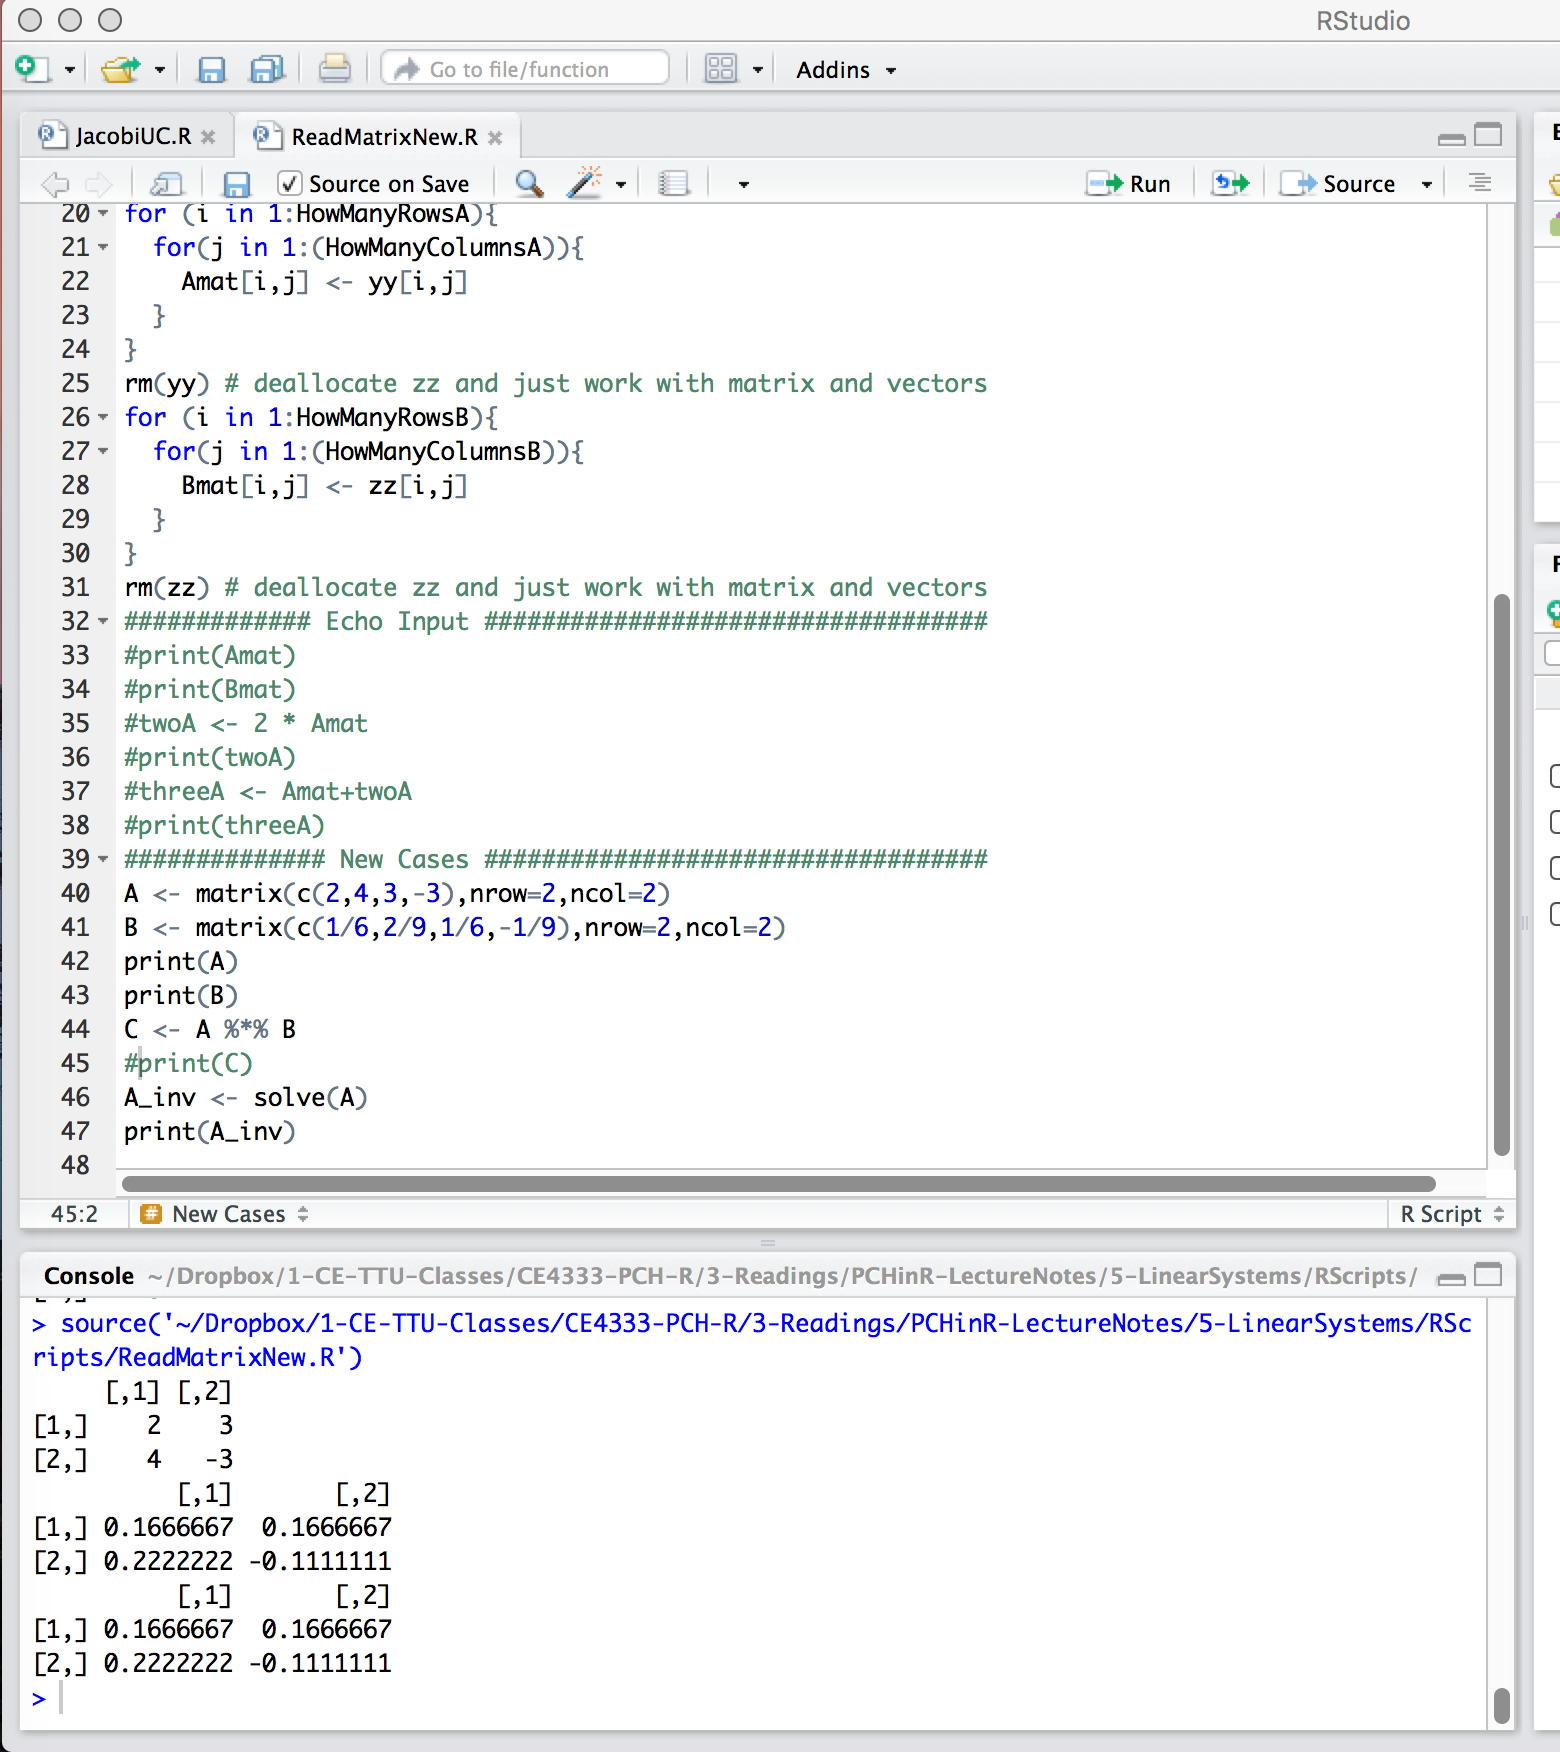
\includegraphics[width=6in]{./5-LinearSystems/InvertedMatrix.jpg} 
   \caption{The matrix inversion script  showing results of a run and various input and output.}
   \label{fig:InvertedMatrix}
\end{figure}
\clearpage


%\subsection{Exercises}
%\begin{enumerate}
%\item Develop a script to read and multiply two matrices.  
%\begin{enumerate}
%\item Apply the script to find $\mathbf{A}\mathbf{x}$ where.
%\begin{gather}
%\mathbf{A} =
%\begin{pmatrix}
%4.0 &  1.5 & 0.7 & 1.2 & 0.5 \\
%1.0 & 6.0 & 0.9 & 1.4 & 0.7 \\
%0.5 & 1.0 & 3.9 & 3.2 & 0.9 \\
%0.2 & 2.0 & 0.2 & 7.5 & 1.9  \\
%1.7 & 0.9 & 1.2 & 2.3 & 4.9 \\
%\end{pmatrix}
%~ \mathbf{x} = 
%\begin{pmatrix}
%0.595194878133 \\
%0.507932173989 \\
%0.831708392507 \\
%0.630365599089 \\ 
%1.03737526565 \\
%\end{pmatrix}
%\end{gather}
%\item Use your matrix multiplication program to demonstrate that the inversion example (the 5X5 system above) does indeed produce an inverse matrix.
%\item Use the matrix multiplication program again to demonstrate that $\mathbf{x} = \mathbf{A}^{-1} \mathbf{b}$ where
%\begin{gather}
%\mathbf{A} =
%\begin{pmatrix}
%4.0 &  1.5 & 0.7 & 1.2 & 0.5 \\
%1.0 & 6.0 & 0.9 & 1.4 & 0.7 \\
%0.5 & 1.0 & 3.9 & 3.2 & 0.9 \\
%0.2 & 2.0 & 0.2 & 7.5 & 1.9  \\
%1.7 & 0.9 & 1.2 & 2.3 & 4.9 \\
%\end{pmatrix}
%~ \mathbf{b} = 
%\begin{pmatrix}
%5.0 \\
%6.0 \\
%7.0 \\
%8.0 \\ 
%9.0 \\
%\end{pmatrix}
%\end{gather}
%\end{enumerate}
%\item Develop a script to solve the following linear system of equations
%\begin{gather}
%\begin{matrix}
%2x_1 & ~-~~2x_2 & ~~+3x_3 \\
%2x_1 & ~+~~1x_2 & ~~-2x_3 \\
%4x_1 & ~-~~1x_2 & ~~-3x_3 \\
%\end{matrix}
%\begin{matrix}
%=~10\\
%=~-2\\
%=~0\\
%\end{matrix}
%\end{gather}
%
%\item Develop a script to solve the following linear system of equations\footnote{This can be a somewhat tricky problem, if you have troubles try to interchange the rows need so that the diagonal is non-zero.  If you use the matrix inverter with the system as presented you will get an error,  but if you rearrange the rows so that the diagonal term is non-zero for each row, then the solver works.  An improved version of the inverter would detect the singular nature and attempt to pivot (swap rows) to generate an investable matrix. If you just solve the system in \textbf{R} it will probably work.}
%\begin{gather}
%\begin{matrix}
%0.866x_1 & 0x_2 & -0.5x_3 & 0x_4 & 0x_5 & 0x_6 \\
%0.5x_1 & 0x_2 & 0.866x_3 & 0x_4 & 0x_5 & 0x_6 \\
%-0.866x_1 & -1x_2 & 0x_3 & -1x_4 & 0x_5 & 0x_6 \\
%-0.5x_1 & 0x_2 & 0x_3 & 0x_4 & -1x_5 & 0x_6 \\
%-0.5x_1 & 0x_2 & 0x_3 & x_4 & x_5 & x_6 \\
%0x_1 & 0x_2 & -0.866x_3 & 0x_4 & 0x_5 & -1x_6 \\
%\end{matrix}
%\begin{matrix}
%=~~~~0\\
%=-1000\\
%=~~~~0\\
%=~~~~0\\
%=~~~~0\\
%=~~~~0\\
%\end{matrix}
%\end{gather}
%
%%\item Develop a program to compute the determinant of a matrix --- apply the program to the coefficient matrix in the previous problem.   
%
%\end{enumerate}
%\subsubsection{Application Project: Static Truss Analysis}
%Figure \ref{fig:StaticTrussSketch} is a simply supported, statically determinate truss with pin connections (zero moment transfer connections).   Find forces in each member for the loading shown.
%\begin{figure}[htbp] %  figure placement: here, top, bottom, or page
%   \centering
%   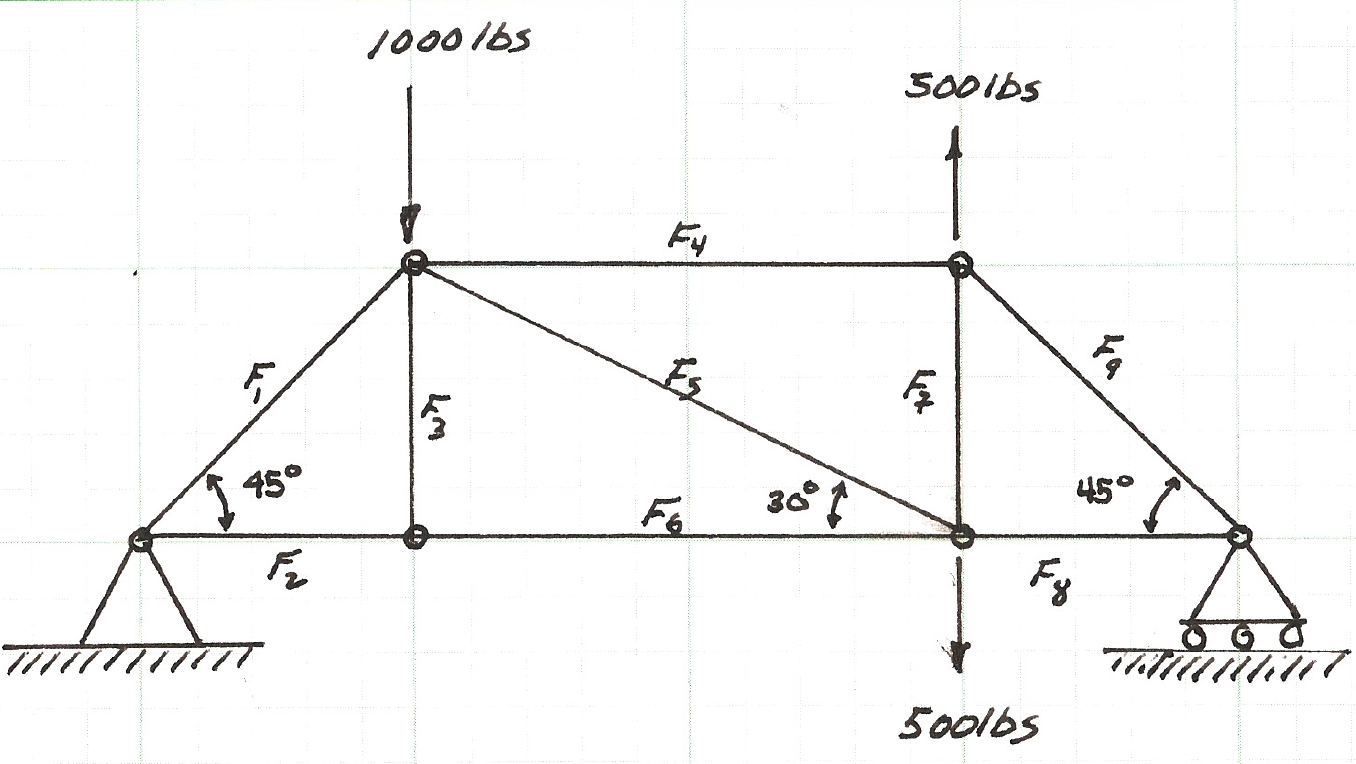
\includegraphics[width=4in]{./5-LinearSystems/StaticTrussSketch.jpg} 
%   \caption{Sketch of simply supported, static truss}
%   \label{fig:StaticTrussSketch}
%\end{figure}
%
%\textsl{Static Analysis}
%Before even contemplating writing/using a program we need to build a mathematical model of the truss and assemble the system of linear equations that result from the model.  So the first step is to sketch a free-body-diagram as in Figure \ref{fig:StaticTrussFBD} and build a node naming convention and force names.
%
%\begin{figure}[h!] %  figure placement: here, top, bottom, or page
%   \centering
%   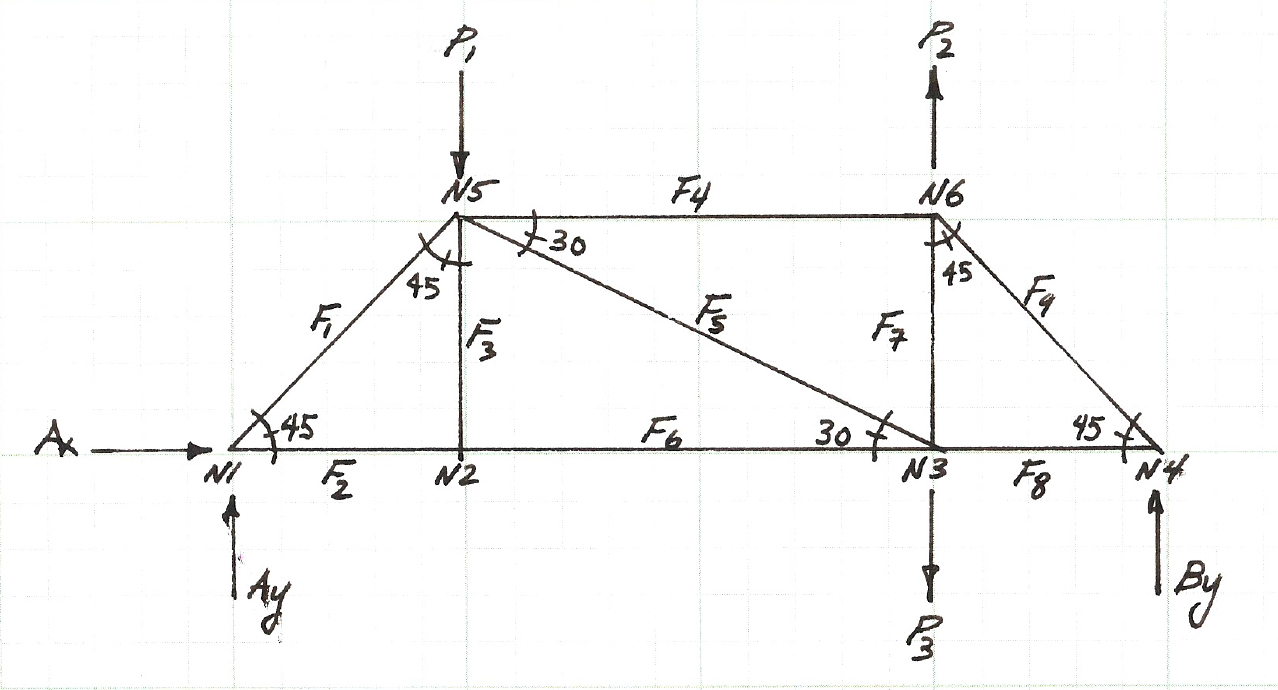
\includegraphics[width=4in]{./5-LinearSystems/StaticTrussFBD.jpg} 
%   \caption{Static truss free-body-diagram showing forces and node naming convention.}
%   \label{fig:StaticTrussFBD}
%\end{figure}
%
%Next we will write the force balance for each of the six nodes ($N1$-$N6$), which will produce a total of 12 equations in the 12 unknowns (the 9 member forces, and 3 reactions).
%\clearpage
%Figure \ref{fig:Node1} is the force balance for node $N1$, the two force equations (for the horizontal, $x$, direction and the vertical, $y$, direction) are listed below the figure.
%\begin{figure}[h!] %  figure placement: here, top, bottom, or page
%   \centering
%   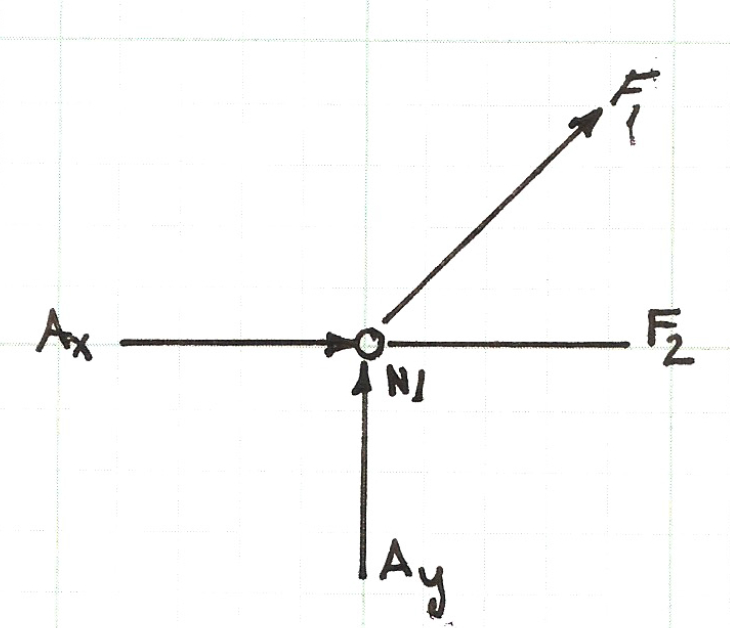
\includegraphics[width=2in]{./5-LinearSystems/Node1.jpg} 
%   \caption{Force diagram at node N1}
%   \label{fig:Node1}
%\end{figure}
%
%\begin{gather}
%\begin{small}
%%\mathbf{A} =
%\begin{matrix}
%\sum F_x = 0 = & +F_1cos(45) & + F_2 &  &  &  &  &  &  & + A_x &  &  & & & \\
%\sum F_y = 0 = & +F_1sin(45) &  & &  &  &  &  &  &  &  & + A_y &  &  & \\
%\end{matrix}
%\end{small}
%\label{eqn:Node1Pair}
%\end{gather}
%
%Equation \ref{eqn:Node1Pair} is the force balance equation pair for the node.  The $x$ component equation will later be named $N1_x$ to indicate it arises from Node 1, $x$ component equation.   A similar notation convention will also be adopted for the $y$ component equation.  There will be an equation pair for each node.
%\begin{figure}[h!] %  figure placement: here, top, bottom, or page
%   \centering
%   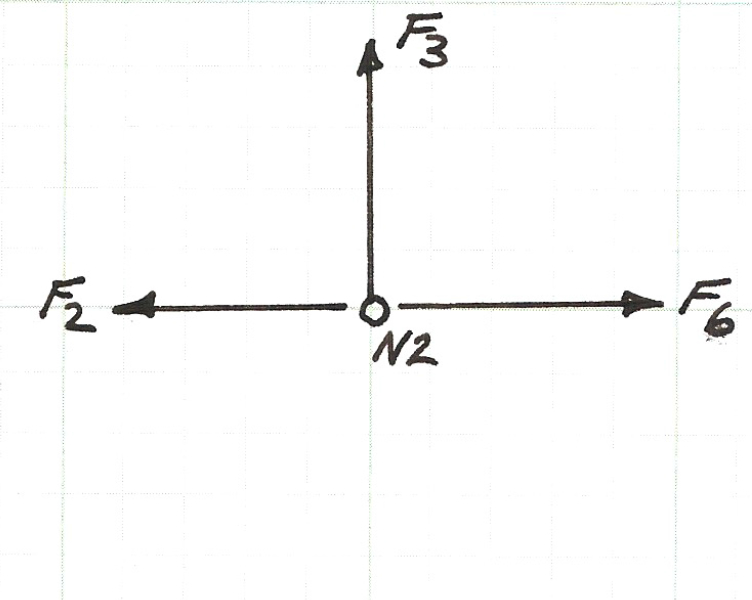
\includegraphics[width=2in]{./5-LinearSystems/Node2.jpg} 
%   \caption{Force diagram at node N2}
%   \label{fig:Node2}
%\end{figure}
%
%\begin{gather}
%\begin{small}
%%\mathbf{A} =
%\begin{matrix}
%\sum F_x = 0 = &  & -F_2 &  &  &  & +F_6 &  &  &  &  &  &  & & \\
%\sum F_y = 0 =  &  &  & +F_3 &  &  &  &  &  &  &  &  &  & & \\
%\end{matrix}
%\end{small}
%\label{eqn:Node2Pair}
%\end{gather}
%Equation \ref{eqn:Node2Pair} is the force balance equation pair for node $N2$.
%\clearpage
%
%\begin{figure}[h!] %  figure placement: here, top, bottom, or page
%   \centering
%   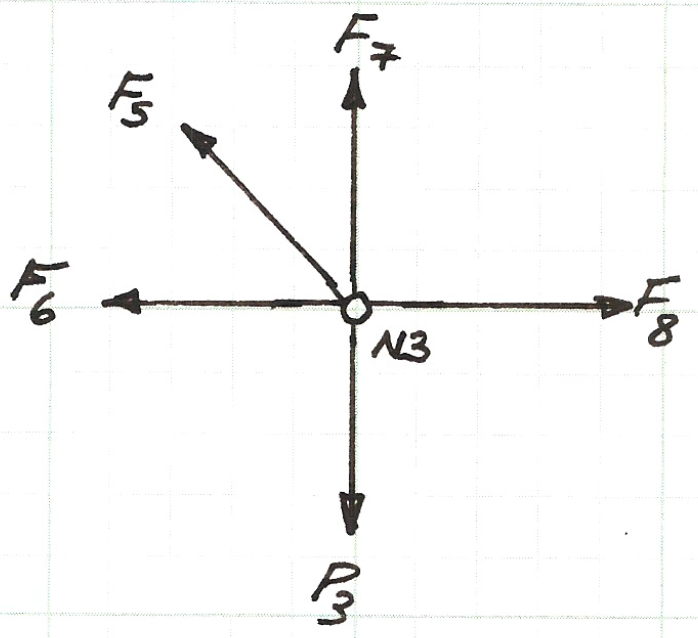
\includegraphics[width=2in]{./5-LinearSystems/Node3.jpg} 
%   \caption{Force diagram at node N3}
%   \label{fig:Node3}
%\end{figure}
%
%\begin{gather}
%\begin{small}
%%\mathbf{A} =
%\begin{matrix}
%\sum F_x = 0 = &  &  &  &  & -F_5cos(30) & -F_6 & & +F_8 &  &  &  &  &  & \\
%\sum F_y = 0 =  &  &  &  &  & F_5sin(30) &  & +F_7 &  &  &  &  &  &  & -P_3\\
%\end{matrix}
%\end{small}
%\label{eqn:Node3Pair}
%\end{gather}
%Equation \ref{eqn:Node3Pair} is the force balance equation pair for node $N3$.
%
%\begin{figure}[h!] %  figure placement: here, top, bottom, or page
%   \centering
%   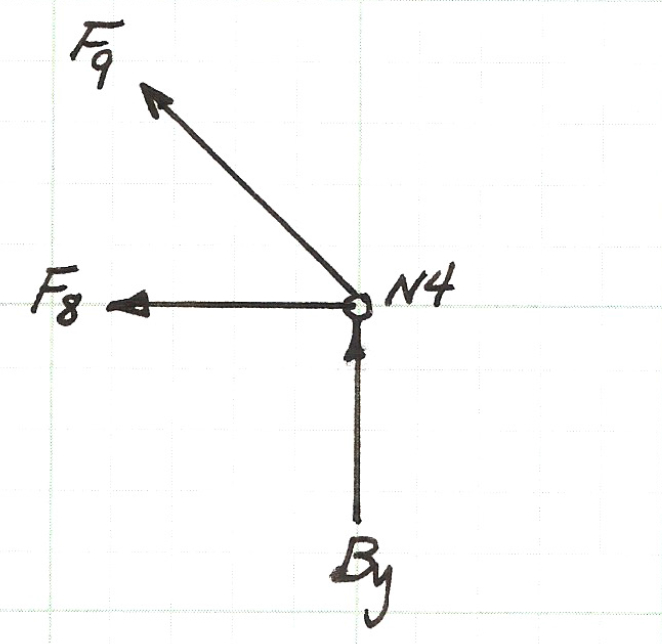
\includegraphics[width=2in]{./5-LinearSystems/Node4.jpg} 
%   \caption{Force diagram at node N4}
%   \label{fig:Node4}
%\end{figure}
%
%\begin{gather}
%\begin{small}
%%\mathbf{A} =
%\begin{matrix}
%\sum F_x = 0 = &  &  &  &  &  &  &  & -F_8 & -F_9cos(45) &  &  &  &  & \\
%\sum F_y = 0 =  &  &  &  &  &  &  &  &  & F_9sin(45) &  &  & +B_y  &  & \\
%\end{matrix}
%\end{small}
%\label{eqn:Node4Pair}
%\end{gather}
%Equation \ref{eqn:Node4Pair} is the force balance equation pair for node $N4$.
%\clearpage
%
%\begin{figure}[h!] %  figure placement: here, top, bottom, or page
%   \centering
%   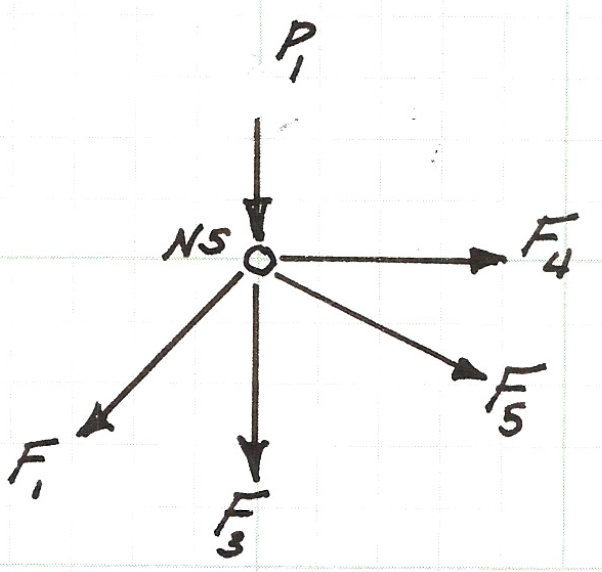
\includegraphics[width=2in]{./5-LinearSystems/Node5.jpg} 
%   \caption{Force diagram at node N5}
%   \label{fig:Node5}
%\end{figure}
%
%\begin{gather}
%\begin{small}
%%\mathbf{A} =
%\begin{matrix}
%\sum F_x = 0 = & -F_1cos(45) &  &   & +F_4 & +F_5cos(30) &  &  &  &  &  &  &  &  & \\
%\sum F_y = 0 =  & -F_1sin(45) &  & -F_3 &   & -F_5sin(30) &  &  &  &  &  &  &  &  & -P_1\\
%\end{matrix}
%\end{small}
%\label{eqn:Node5Pair}
%\end{gather}
%Equation \ref{eqn:Node5Pair} is the force balance equation pair for node $N5$.
%
%\begin{figure}[h!] %  figure placement: here, top, bottom, or page
%   \centering
%   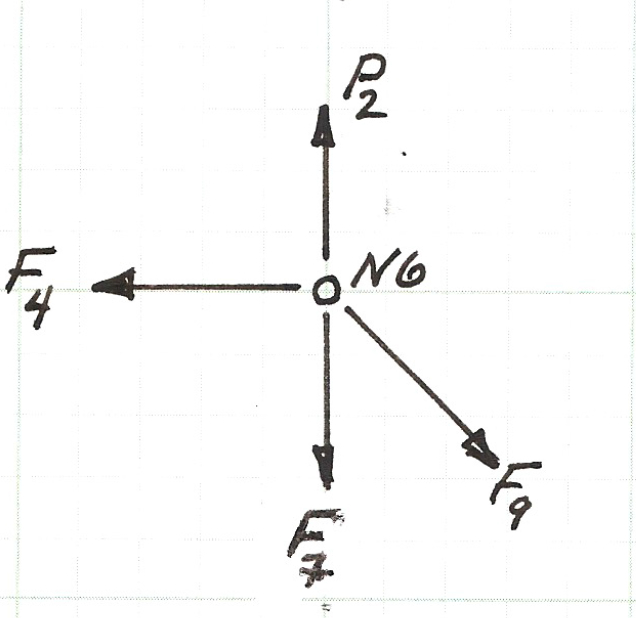
\includegraphics[width=2in]{./5-LinearSystems/Node6.jpg} 
%   \caption{Force diagram at node N6}
%   \label{fig:Node6}
%\end{figure}
%\begin{gather}
%\begin{small}
%%\mathbf{A} =
%\begin{matrix}
%\sum F_x = 0 = &  &  &  & -F_4 &  &  &  &  & F_9sin(45) &  &  &  &  & \\
%\sum F_y = 0 =  &  &  &  &  &  &  & -1 &  & -F_9cos(45) &  &  &  &  & P_2\\
%\end{matrix}
%\end{small}
%\label{eqn:Node6Pair}
%\end{gather}
%Equation \ref{eqn:Node6Pair} is the force balance equation pair for node $N6$.
%\clearpage
%
%The next step is to gather the equation pairs into a system of linear equations.   We will move the known loads to the right hand side and essentially construct the matrix equation $\mathbf{A}\mathbf{x} = \mathbf{b}$.   Equation \ref{eqn:AugmentTrussMatrix} is a matrix representation of the equation pairs with the forces moved to the right hand side $\mathbf{b} = RHS$. 
%\begin{gather}
%\begin{small}
%%\mathbf{A} =
%\begin{pmatrix}
%~ & F_1 & F_2 & F_3 & F_4 & F_5 & F_6 & F_7 & F_8 & F_9 & A_x & A_y & B_y & | & RHS\\
%\hline
%N1_x & 0.707 & 1 & 0 & 0 & 0 & 0 & 0 & 0 & 0 & 1 & 0 & 0 & | & 0\\
%N1_y & 0.707 & 0 & 0 & 0 & 0 & 0 & 0 & 0 & 0 & 0 & 1 & 0 & | & 0\\
%N2_x & 0 & -1 & 0 & 0 & 0 & 1 & 0 & 0 & 0 & 0 & 0 & 0 & | & 0\\
%N2_y & 0 & 0 & 1 & 0 & 0 & 0 & 0 & 0 & 0 & 0 & 0 & 0 & | & 0\\
%N3_x & 0 & 0 & 0 & 0 & -0.866 & -1 & 0 & 1 & 0 & 0 & 0 & 0 & | & 0\\
%N3_y & 0 & 0 & 0 & 0 & 0.5 & 0 & 1 & 0 & 0 & 0 & 0 & 0 & | & P_3\\
%N4_x & 0 & 0 & 0 & 0 & 0 & 0 & 0 & -1 & -0.707 & 0 & 0 & 0 & | & 0\\
%N4_y & 0 & 0 & 0 & 0 & 0 & 0 & 0 & 0 & 0.707 & 0 & 0 & 0 & | & 0\\
%N5_x & -0.707 & 0 & 0 & 1 & 0.866 & 0 & 0 & 0 & 0 & 0 & 0 & 0 & | & 0\\
%N5_y & -0.707 & 0 & -1 & 0 & -0.5 & 0 & 0 & 0 & 0 & 0 & 0 & 0 & | & P_1\\
%N6_x & 0 & 0 & 0 & -1 & 0 & 0 & 0 & 0 & 0.707 & 0 & 0 & 0 & | & 0\\
%N6_y & 0 & 0 & 0 & 0 & 0 & 0 & -1 & 0 & -0.707 & 0 & 0 &  0 & | & -P_2\\
%\end{pmatrix}
%\end{small}
%\label{eqn:AugmentTrussMatrix}
%\end{gather}
%
%In Equation \ref{eqn:AugmentTrussMatrix}, the rows are labeled on the left-most column with their node-related equation name.   Thus each row of the matrix corresponds to an equation derived from a node.   The columns are labeled with their respective unknown force (except the last column, which represents the right-hand-side of the system of linear equations).  Thus the coefficient in each column corresponds to a force in each node equation.   The sign of the coefficient refers to the assumed direction the force acts.   In the analysis all the members were assumed to be in tension (except for the reaction forces).   If a coefficient has a value of zero in a particular row, then than force does no act at the node to which the row corresponds.    
%
%From this representation the transition to the formal vector-matrix representation is straightforward.  Equation \ref{eqn:TrussMatrix}, Equation \ref{eqn:TrussX}, Equation \ref{eqn:TrussRHS} are the $\mathbf{A}$ matrix, the $\mathbf{x}$ vector, and the $\mathbf{b}$ vector, respectively.
%
%Finally, like the last problem in the exercises, the rows need to be re-ordered so the main diagonal contains non-zero values before attempting to solve the linear system.   The remaining project task is to rearrange the rows (by-hand is fine, although writing code to generate an ordering would be a worthy endeavor!), then find the unknown forces using the matrix routines we have already constructed.\footnote{In a later chapter full pivoting will be presented, and with full pivoting this system can be solved without the human having to rearrange rows.}   
%
%One pretty cool feature of this analysis, is we solve for the reactions without needing to know member lengths (no moments).  
%
%\begin{gather}
%\begin{small}
%\mathbf{A} =
%\begin{pmatrix}
%0.707 & 1 & 0 & 0 & 0 & 0 & 0 & 0 & 0 & 1 & 0 & 0 \\
%0.707 & 0 & 0 & 0 & 0 & 0 & 0 & 0 & 0 & 0 & 1 & 0 \\
%0 & -1 & 0 & 0 & 0 & 1 & 0 & 0 & 0 & 0 & 0 & 0 \\
%0 & 0 & 1 & 0 & 0 & 0 & 0 & 0 & 0 & 0 & 0 & 0 \\
%0 & 0 & 0 & 0 & -0.866 & -1 & 0 & 1 & 0 & 0 & 0 & 0 \\
%0 & 0 & 0 & 0 & 0.5 & 0 & 1 & 0 & 0 & 0 & 0 & 0 \\
%0 & 0 & 0 & 0 & 0 & 0 & 0 & -1 & -0.707 & 0 & 0 & 0 \\
%0 & 0 & 0 & 0 & 0 & 0 & 0 & 0 & 0.707 & 0 & 0 & 0 \\
%-0.707 & 0 & 0 & 1 & 0.866 & 0 & 0 & 0 & 0 & 0 & 0 & 0 \\
%-0.707 & 0 & -1 & 0 & -0.5 & 0 & 0 & 0 & 0 & 0 & 0 & 0 \\
%0 & 0 & 0 & -1 & 0 & 0 & 0 & 0 & 0.707 & 0 & 0 & 0 \\
%0 & 0 & 0 & 0 & 0 & 0 & -1 & 0 & -0.707 & 0 & 0 &  0 \\
%\end{pmatrix}
%\end{small}
%\label{eqn:TrussMatrix}
%\end{gather}
%
%\begin{gather}
%\begin{small}
%\mathbf{x} =
%\begin{pmatrix}
%F_1\\
%F_2\\
%F_3\\
%F_4\\
%F_5\\
%F_6\\
%F_7\\
%F_8\\
%F_9\\
%A_x\\
%A_y\\
%B_y\\
%\end{pmatrix}
%\end{small}
%\label{eqn:TrussX}
%\end{gather}
%
%\begin{gather}
%\begin{small}
%\mathbf{b} =
%\begin{pmatrix}
%0\\
%0\\
%0\\
%0\\
%0\\
%P_3\\
%0\\
%0\\
%0\\
%P_1\\
%0\\
%-P_2\\
%\end{pmatrix}
%\end{small}
%\label{eqn:TrussRHS}
%\end{gather}
%
%Using your scripts from the Exercises,  the resulting linear system and determine the forces in each member.

%%%%%%%%%%%%%%%%%%%%%%%%%%%%%%%%%%%%%%%%%%%%%%%%%%%%%%%%%%%%%%%
\subsection{Jacobi Iteration -- An iterative method to find solutions}
Iterative methods are often more rapid and economical in storage requirements than the direct methods in \texttt{solve(\dots)}.\footnote{The \textbf{R} solve routine is pretty robust, if you tell it \texttt{sparse=TRUE} it has a lot of internal methods to pre-condition the problem for fast solution.  But for really big systems we may wish to program our own solver --- especially if these systems have some special and predictable structure.}  The methods are useful (necessary) for non-linear systems of equations --- we will use this feature later when we find solutions to networks of pipelines.  

Lets consider a simple example:
\begin{gather}
\begin{matrix}
8 x_1 & +~1 x_2 & -~1 x_3  \\
1 x_1 & -~7 x_2 &  +~2 x_3 \\
2 x_1 & +~1 x_2 & +~9 x_3  \\
\end{matrix}
\begin{matrix}
=~~~~8\\
=~-4\\
=~~~12\\
\end{matrix}
\end{gather}

The solution is $x_1 = 1$, $x_2 = 1$, $x_3 = 1$.  
We begin the iterative scheme by refactoring each equation in terms of a single variable (there is a secret pivot step to try to make the system diagonally dominant -- the example above has already been pivoted, or ``pre-conditioned'' for the solution method):

\begin{gather}
\begin{matrix}
x_1 \\
x_2 \\
x_3  \\
\end{matrix}
\begin{matrix}
=~ 1.000 & ~ & -0.125 x_2 & 0.125 x_3 \\
=~ 0.571 & 0.143 x_1  & ~ & 0.286 x_3 \\
=~ 1.333 & -0.222 x_1 & -0.111 x_2 & ~ \\
\end{matrix}
\end{gather}

Then supply an initial guess of the solution (e.g. $(0,0,0)$) and put these values into the right-hand side, the resulting left-hand side is an improved (hopefully) solution.
Repeat the process until the solution stops changing, or goes obviously haywire.

This sequence of operation for the example above produces the results listed in Table \ref{tab:jacobi}.

% Requires the booktabs if the memoir class is not being used
\begin{table}[h!]
   \centering
      \caption{Jacobi Iteration Solution Sequence}
   \begin{tabular}{lllllllll} % Column formatting, @{} suppresses leading/trailing space
      \toprule
Iteration:&1-st&2-nd&3-rd&4-th&5th&6-th&7-th&8-th\\
\hline
$x_1$&0&1.000&1.095&0.995&0.993&1.002&1.001&1.000\\
$x_2$&0&0.571&1.095&1.026&0.990&0.998&1.001&1.000\\
$x_3$&0&1.333&1.048&0.969&1.000&1.004&1.001&1.000\\
      \bottomrule
   \end{tabular}
   \label{tab:jacobi}
\end{table}

As a practical matter, refactoring the equations can instead be accomplished by computing the inverse of each diagonal coefficient -- and matrix multiplication, scalar division, and vector addition are all that is required to find a solution (if the method will actually work).

In linear algebra terms the Jacobi iteration method (without refactoring) performs the following steps:
\begin{enumerate}
\item Read in $\mathbf{A}$, $\mathbf{b}$, and $\mathbf{x_{guess}}$.
\item Construct a vector from the diagonal elements of $\mathbf{A}$.  This vector, $\mathbf{W}$, will have one column, and same number of rows as $\mathbf{A}$.
\item Perform matrix arithmetic to compute an error vector, $\mathbf{residual}=\mathbf{A} \cdot \mathbf{x_{guess}} - \mathbf{b}$.
\item Divide this error vector by the diagonal weights $\mathbf{update} = \mathbf{residual} / \mathbf{W}$
\item Update the solution vector $\mathbf{x_{new}} = \mathbf{x_{guess}} - \mathbf{update}$
\item Test for stopping, if not indicated, move the new solution into the guess and return to step 3.
\item If time to stop, then report result and stop.
\end{enumerate}
Listing \ref{lst:JacobiUC} implements in \textbf{R} the algorithm described above to find solutions by the Jacobi iteration method. 
The script does not pre-condition the linear system (so we have to do that ourselves).

\begin{lstlisting}[caption=R code demonstrating Jacobi Iteration , label=lst:JacobiUC]
# R script to implement Jacobi Iteration Method to 
#   find solution to simultaneous linear equations
#   assumes matrix is pre-conditioned to diagional dominant
#   assumes matrix is non-singular
############## READ IN DATA FROM A FILE ####################
filepath <- "~/Dropbox/1-CE-TTU-Classes/CE4333-PCH-R/3-Readings/PCHinR-LectureNotes/5-LinearSystems/RScripts"
filename <- "LinearSystem000.txt"
fileToRead <- paste(filepath,filename,sep="/") # build the user absolute filename
# Here we open the connection to the file (within read.table)
# Then the read.table attempts to read the entire file into an object named zz
# Upon either fail or success, read.table closes the connection
zz <- read.table(fileToRead,header=FALSE,sep=",") # comma seperated ASCII, No header
############## Row and Column Counts #######################
HowManyColumns <- length(zz)
HowManyRows    <- length(zz$V1)
tolerance <- 1e-12 #stop when error vector is small
itermax <- 200 # maximum number of iterations
############### Build A, x, and B ##############################
Amat <- matrix(0,nrow = HowManyRows, ncol = (HowManyColumns-2) )
xguess <- numeric(0)
Bvec <- numeric(0)
Wvec <- numeric(0)
############################################################
for (i in 1:HowManyRows){
  for(j in 1:(HowManyColumns-2)){
    Amat[i,j] <- zz[i,j]
  }
  Bvec[i] <- zz[i,HowManyColumns-1]
  xguess[i] <- zz[i,HowManyColumns]
  Wvec[i] <- Amat[i,i]
}
rm(zz) # deallocate zz and just work with matrix and vectors 
#####################Implement Jacobi Iteration #############
for(iter in 1:itermax){
Bguess <- Amat %*% xguess
residue <- Bguess - Bvec
xnew <- xguess - residue/Wvec
xguess <- xnew
testval <- t(residue) %*% residue
if (testval < tolerance) {
  message("sum squared error vector small : ",testval);
  break
}
}
if( iter == itermax) message("Method Fail")
message(" Number Iterations : ", iter)
message(" Coefficient Matrix : ")
print(cbind(Amat))
message(" Solution Vector : ")
print(cbind(xguess))
message(" Right-Hand Side Vector : ")
print(cbind(Bvec))
\end{lstlisting}

Figure \ref{fig:JacobiUC-Works} is a screen capture of the script in Listing \ref{lst:JacobiUC} applied to the example problem.

\begin{figure}[h!] %  figure placement: here, top, bottom, or page
   \centering
   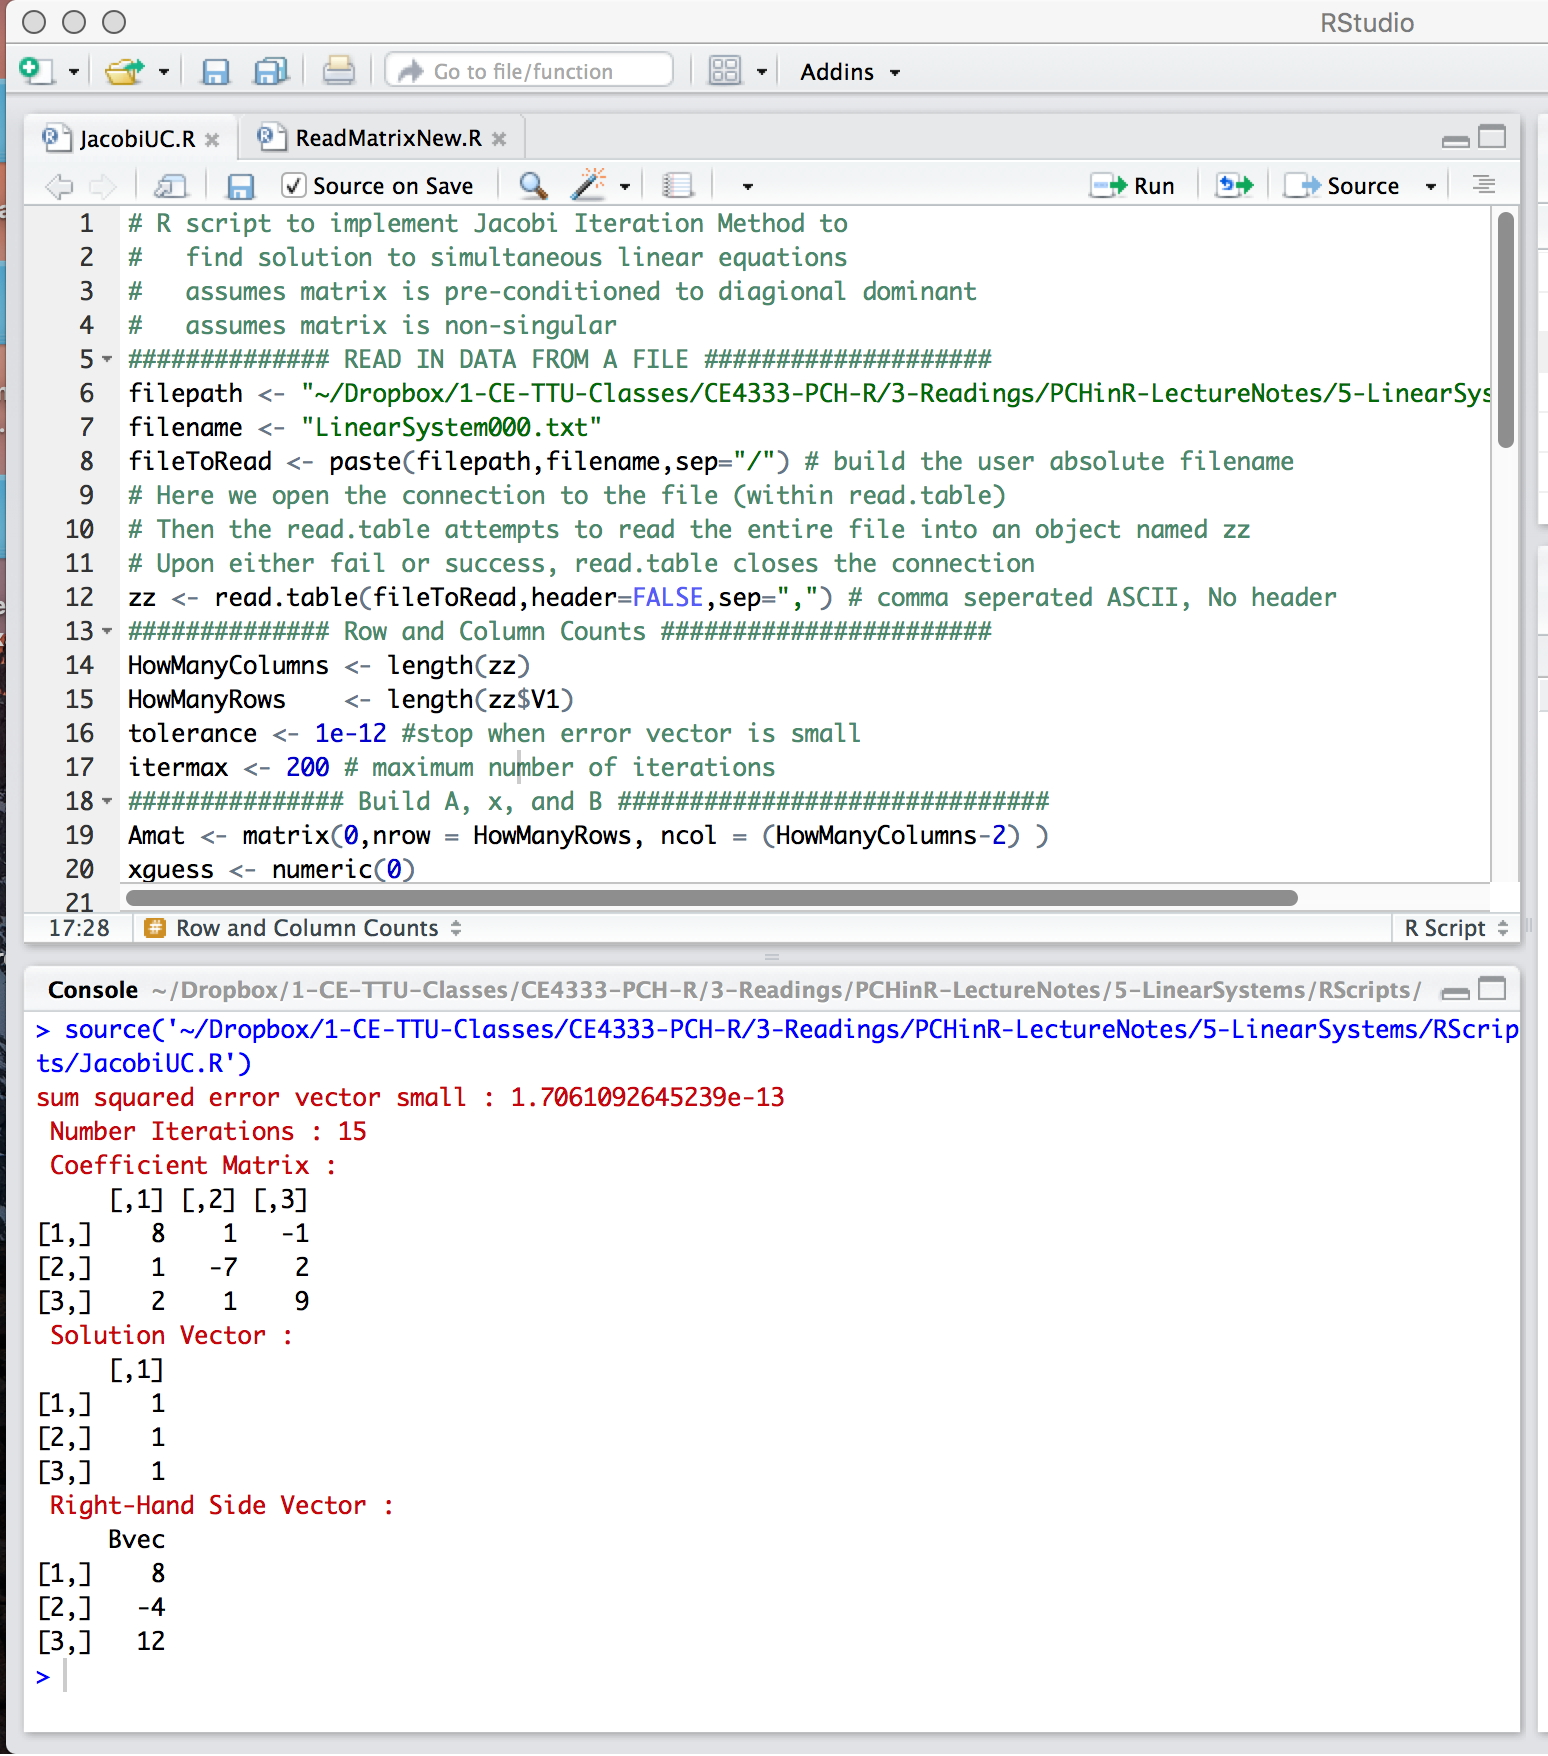
\includegraphics[width=6in]{./5-LinearSystems/JacobiUC-Works.jpg} 
   \caption{Jacobi Iteration applied to Example Problem}
   \label{fig:JacobiUC-Works}
\end{figure}
\clearpage
%\subsection{Exercises}
%\begin{enumerate}
%\item Develop a script to implement the Jacobi iteration method.  
%\item Apply your Jacobi script to find $\mathbf{x}$ in $\mathbf{A} \cdot \mathbf{x} = \mathbf{b}$ where.
%\begin{gather}
%\mathbf{A} =
%\begin{pmatrix}
% ~5 & -1 &  ~0 \\
%-1 &  ~5 & -1 \\
% ~0 & -1 &  ~5 \\
%\end{pmatrix}
%~ \mathbf{B} = 
%\begin{pmatrix}
%~9 \\
%~4 \\
%-6 \\
%\end{pmatrix}
%\end{gather}
%\item Solve the same system using \texttt{solve(\dots)} in \textbf{R}. 
%\item \label{prob:jacobiPass} Apply your Jacobi script to find $\mathbf{x}$ in $\mathbf{A} \cdot \mathbf{x} = \mathbf{b}$ where.
%\begin{gather}
%\mathbf{A} =
%\begin{pmatrix}
%1.48 &  0.93 & -1.30\\
%2.68 &  3.04 & -1.48\\
%2.51 &  1.48 &  4.53\\
%\end{pmatrix}
%~ \mathbf{b} = 
%\begin{pmatrix}
%1.03\\
%-0.53\\ 
%0.05\\
%\end{pmatrix}
%\end{gather}
%\item Solve the same system using \texttt{solve(\dots)} in \textbf{R}. 
%\item \label{prob:jacobiFail} Apply your Jacobi script to find $\mathbf{x}$ in $\mathbf{A} \cdot \mathbf{x} = \mathbf{b}$ where.
%\begin{gather}
%\mathbf{A} =
%\begin{pmatrix}
%2.51 &  1.48 &  4.53\\
%1.48 &  0.93 & -1.30\\
%2.68 &  3.04 & -1.48\\
%\end{pmatrix}
%~ \mathbf{b} = 
%\begin{pmatrix}
%0.05\\
%1.03\\
%-0.53\\ 
%\end{pmatrix}
%\end{gather}
%\item Solve the same system using \texttt{solve(\dots)} in \textbf{R}. 
%\item Problem \ref{prob:jacobiFail} failed using Jacobi -- however it is identical in a linear algebra sense to Problem \ref{prob:jacobiPass}.  
%How should the system have been pre-conditioned before attempting the Jacobi solution?\footnote{An internet search on pre-conditioning would be helpful in answering this problem.}
%
%
%
%%\item Develop a program to compute the determinant of a matrix --- apply the program to the coefficient matrix in the previous problem.   
%
%\end{enumerate}
